\documentclass[a4paper, 12pt]{article}
\usepackage[left=2.5cm, right=2.5cm, top=3cm, bottom=3cm]{geometry}
\usepackage[spanish]{babel}
\usepackage{amsmath}
\usepackage{graphicx}
\usepackage{color}
\usepackage{xcolor}
\usepackage[utf8]{inputenc}
\usepackage[T1]{fontenc}
\usepackage{listings}
\usepackage{tikz}
\usetikzlibrary{shapes,arrows,positioning}
\usepackage{float}




\definecolor{colorgreen}{rgb}{0,0.6,0}
\definecolor{colorgray}{rgb}{0.5,0.5,0.5}
\definecolor{colorpurple}{rgb}{0.58,0,0.82}
\definecolor{colorback}{RGB}{255,255,204}
\definecolor{colorbackground}{RGB}{200,200,221}
%Definiendo el estilo de las porciones de codigo
\lstset{
backgroundcolor=\color{colorbackground},
commentstyle=\color{colorgreen},
keywordstyle=\color{colorpurple},
numberstyle=\tiny\color{colorgray},
stringstyle=\color{colorgreen},
basicstyle=\ttfamily\footnotesize,
breakatwhitespace=false,
breaklines=true,
captionpos=b,
keepspaces=true,
numbers=left,
showspaces=false,
showstringspaces=false,
showtabs=false,
tabsize=2,
frame=single,
framesep=2pt,
rulecolor=\color{black},
framerule=1pt
}



\begin{document}
\graphicspath{{./}}

\begin{center}
\text{\huge Análisis estadístico de datos}\\
\vspace {1cm}
\text{\huge Dataset: Accidentes cerebrovascular}\\

\begin{figure}[h]
    \centering
    \includegraphics[width=0.9\textwidth]{img/Presentación.jpg}
\end{figure}

\text{\Large Integrantes:}\\
\begin{itemize}
\centering
\item Eveliz Espinaco Milián
\item Michell Viu Ramirez
\item Dayan Cabrera Leal
\end{itemize}
\vspace {0.5cm}
\text{\Large Grupo 311, Ciencia de la computación,}\\
\text{\Large Facultad de Matemática y Computación, Universidad de La Habana}\\
\text{Curso 2024-2025}

\begin{figure}[h]
    \centering
    
\includegraphics[width=0.2\textwidth]{img/MATCOM.jpg}
\end{figure}



\end{center}

\newpage
\tableofcontents

\newpage
\section{Descripción del problema}
El término accidente cerebrovascular (ACV) engloba dos afecciones médicas distintas: los infartos cerebrales y los derrames cerebrales. Los infartos cerebrales, también conocidos como isquemia cerebral, ocurren cuando hay una reducción significativa y repentina del flujo sanguíneo hacia una región del cerebro, lo que resulta en una privación de oxígeno y nutrientes esenciales para las células cerebrales. Esta falta de flujo sanguíneo provoca la muerte celular en el área afectada, generando daños permanentes en las funciones cerebrales. Por otro lado, los derrames cerebrales o hemorragias cerebrales son causados por la ruptura de un vaso sanguíneo en el cerebro, lo que provoca sangrado dentro del tejido cerebral, con efectos igualmente graves.

Según la Organización Mundial de la Salud (OMS), los accidentes cerebrovasculares, junto con las enfermedades de las arterias coronarias, constituyen las principales enfermedades cardiovasculares responsables de millones de muertes anuales en todo el mundo. Estas patologías representan una de las principales causas de morbilidad a nivel global, lo que subraya la necesidad urgente de prevención, diagnóstico temprano y tratamiento eficaz.

El presente informe tiene como objetivo realizar un análisis estadístico utilizando técnicas de estadística descriptiva e inferencia estadística para predecir la probabilidad de que un paciente sufra un accidente cerebrovascular. El análisis se llevará a cabo tomando en cuenta diversos factores como el sexo, la edad, antecedentes de enfermedades y el tabaquismo, entre otros. Para ello, se utilizará una muestra de 200 individuos. El dataset consta de 200 registros (filas) y 11 variables (columnas). Cada fila en el conjunto de datos proporciona información clave sobre una persona, lo que permite realizar un análisis profundo sobre los factores de riesgo asociados con los accidentes cerebrovasculares.

Este enfoque estadístico busca ofrecer predicciones precisas que ayuden a identificar a individuos con mayor riesgo de sufrir un accidente cerebrovascular, contribuyendo a mejorar las estrategias preventivas y de intervención temprana.

\newpage
\section{Variables Estadísticas}
A continuación, se describen las variables incluidas en el dataset, detallando su significado, los valores que pueden tomar, y su clasificación correspondiente.

\begin{enumerate}

\item \textbf{Sexo:} Indica el sexo del paciente.
    \begin{itemize}
    \item Valores posibles: 0 Mujer; 1 Hombre
    \item Clasificación: Según el tipo de dato se clasifica en una \textbf{variable cualitativa nominal}.
    \end{itemize}
\item \textbf{Edad:}  Representa la edad del paciente en años.
    \begin{itemize}
    \item Valores posibles: Enteros positivos
    \item Clasificación: Según el tipo de dato se clasifica en una \textbf{variable cuantitativa discreta}. La escala de medición de la variable es \textbf{de razón}.
    \end{itemize}
\item \textbf{Hipertensión:}  Indica si el paciente ha tenido diagnóstico de hipertensión arterial en algún momento.
    \begin{itemize}
    \item Valores posibles: 0 No ha tenido hipertensión; 1 Ha tenido hipertensión
    \item Clasificación: Según el tipo de dato se clasifica en una \textbf{variable cualitativa nominal}.
    \end{itemize}
\item \textbf{Cardiopatía:} Refleja si el paciente padece alguna enfermedad del corazón.
    \begin{itemize}
    \item Valores posibles: 0 No presenta patologías cardíacas; 1 Presenta patologías cardíacas
    \item Clasificación:Según el tipo de dato se clasifica en una \textbf{variable cualitativa nominal}.
    \end{itemize}
\item \textbf{Casado:} Señala el estado civil del paciente.
    \begin{itemize}
    \item Valores posibles: 0 No está casado; 1 Está casado
    \item Clasificación: Según el tipo de dato se clasifica en una \textbf{variable cualitativa nominal}.
    \end{itemize}
\item \textbf{Tipo de Trabajo:} Describe el tipo de ocupación o situación laboral del paciente.
    \begin{itemize}
    \item Valores posibles:
    \\
    0: Nunca ha trabajado
    \\
    1: Trabajo eventual
    \\
    2: Trabajo estatal
    \\
    3: Trabajo por cuenta propia
    \item Clasificación: Según el tipo de dato se clasifica en una \textbf{variable cualitativa nominal}.
    \end{itemize}
\item \textbf{Tipo de Residencia:} Indica el área de residencia del paciente.
    \begin{itemize}
    \item Valores posibles: 0 Urbana, 1 Rural
    \item Clasificación: Según el tipo de dato se clasifica en una \textbf{variable cualitativa nominal}.
    \end{itemize}
\item \textbf{Nivel Promedio de Glucosa:} Muestra el nivel promedio de azúcar en sangre del paciente en mg/dl (miligramos por decilitro).
    \begin{itemize}
    \item Valores posibles: reales positivos
    \item Clasificación: Según el tipo de dato se clasifica en una \textbf{variable cuantitativa continua}. La escala de medición de la variable es \textbf{de razón}.
    \end{itemize}
\item \textbf{Índice de Masa Corporal (IMC):} Representa el Índice de Masa Corporal del paciente.
    \begin{itemize}
    \item Valores posibles: reales positivos
    \item Clasificación: Según el tipo de dato se clasifica en una \textbf{variable cuantitativa continua}. La escala de medición de la variable es \textbf{de razón}.
    \end{itemize}
\item \textbf{Tabaquismo:} Indica si el paciente es fumador.
    \begin{itemize}
    \item Valores posibles: 0 No fuma, 1 Fuma
    \item Clasificación: Según el tipo de dato se clasifica en una \textbf{variable cualitativa nominal}.
    \end{itemize}
\item \textbf{Accidentes:} Guarda la información de si el paciente a sufrido o no accidentes cerebrovasculares.   
    \begin{itemize}
    \item Valores posibles: 0 El paciente a sufrido accidentes cerebrovasculares, 1 en caso contrario.
    \item Clasificación: Según el tipo de dato se clasifica en una \textbf{variable cualitativa nominal}.
    \end{itemize}

\end{enumerate}

\newpage
\section{Estadísticos de centro}
Los estadísticos de centro tratan de ubicar la posición central del conjunto de valores
para entender la distribución de los datos y detectar posibles valores atípicos. La
siguiente tabla muestra el resultado de calcular cada uno de ellos en cada una de las
variables cuantitativas

\begin{figure}[h]
    \centering
    \includegraphics[width=0.9\textwidth]{img/Tablas/Estadísticos_de_centro.png}
\end{figure}

En la tabla se observa que los valores de la media (60.43) y la mediana (61) para la variable edad son muy cercanos, 
así como los valores del primer cuartil (58) y del tercer cuartil (63). Esto indica que la muestra está compuesta 
principalmente por personas de edad avanzada, entre 58 y 63 años, con una distribución de edades centrada alrededor 
de los 61 años. Esto sugiere una muestra relativamente homogénea en términos de edad, con una posible ausencia de 
valores atípicos extremos.

El nivel promedio de glucosa en sangre en ayunas de una persona saludable se encuentra entre 70 y 100 mg/dL 
(menos del 5.7\%). Valores entre 100 y 125 mg/dL en ayunas se consideran prediabetes, y niveles superiores a 126 mg/dL 
(6.5\% o más) diagnostican a una persona como diabética. Con esta información, podemos observar que la muestra analizada 
incluye personas con niveles de glucosa en sangre que varían entre 79.19 y 188.38 mg/dL, abarcando tanto niveles normales 
como altos. La media de 123.71 mg/dL sugiere que, en promedio, los niveles de glucosa en sangre en la muestra son 
relativamente altos. La mediana de 93.89 mg/dL indica que la distribución de los niveles de glucosa en sangre está centrada 
alrededor de este valor. Además, la media significativamente superior a la mediana sugiere la presencia de algunos valores 
atípicos extremadamente altos que elevan el promedio. La alta dispersión entre el primer y tercer cuartil indica una 
variabilidad considerable en los niveles de glucosa en sangre.

Los valores del índice de masa corporal (IMC) se clasifican generalmente en: bajo peso (IMC menor de 18.5), peso normal 
(IMC entre 18.5 y 24.9), sobrepeso (IMC entre 25 y 29.9) y obesidad (IMC de 30 o mayor). Conociendo estas categorías, 
podemos precisar las características de nuestra muestra respecto a la variable IMC. Observamos que la mayoría de los 
valores en la muestra se encuentran en el rango de 24.45 a 32.05, lo que indica que estamos analizando principalmente 
personas con sobrepeso y obesidad. La media y la mediana sugieren una tendencia hacia el sobrepeso en las personas 
de las observaciones. La diferencia entre el primer cuartil (24.45) y el tercer cuartil (32.05) indica una dispersión 
moderada en los valores de IMC.

\newpage
\section{Estadísticos de dispersión}
Los estadísticos de variabilidad, también conocidos como medidas de dispersión, son
indicadores que describen cuán dispersos o agrupados están los datos del conjunto. La siguiente tabla muestra el resultado de calcular cada uno de ellos en cada una de
las variables cuantitativas.

\begin{figure}[h]
    \centering
    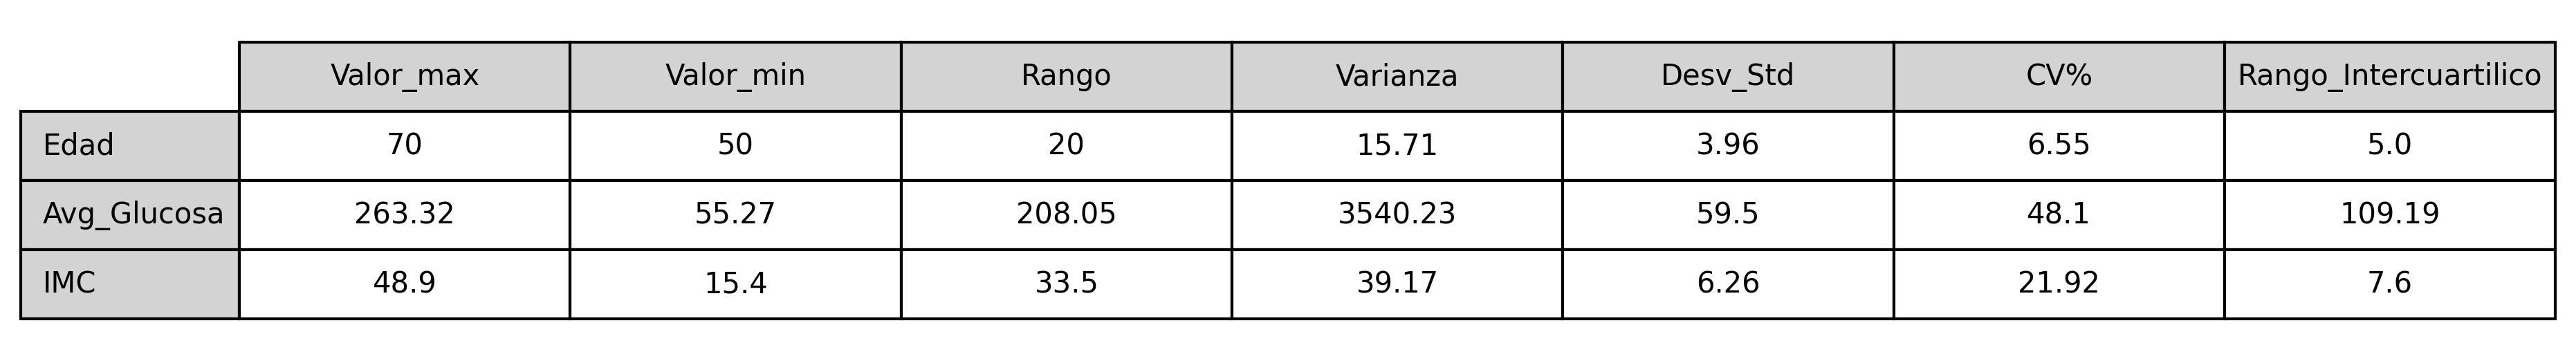
\includegraphics[width=0.9\textwidth]{img/Tablas/Estadísticos_de_dispersión.png}
\end{figure}

Con el resultado del rango podemos tener una idea básica de la dispersión de los datos, pero sin considerar cómo están 
distribuidos los valores restantes, a diferencia de la desviación estándar y el rango intercuartílico. La desviación estándar 
proporciona una medida más detallada de la dispersión de los datos respecto a la media, y el rango intercuartílico indica qué 
tan agrupados están los datos respecto a la mediana.

Los resultados de los estadísticos de dispersión de la variable edad, junto con los estadísticos de centro, nos permiten 
concluir que la muestra analizada presenta una distribución de edades bastante simétrica y concentrada alrededor de la mediana 
de 61 años, con una variabilidad moderada. Los valores de la varianza, la desviación estándar y el coeficiente de variabilidad 
son relativamente bajos, indicando que estamos en presencia de una distribución homogénea. El rango intercuartílico, comparado con el rango total, sugiere que, aunque hay una diferencia de 20 
años entre el individuo más joven y el más viejo, la mayoría de los datos están concentrados en un rango de 5 años alrededor 
de la mediana.

En la variable Nivel Promedio de Glucosa, se observan altos valores en las medidas de dispersión, lo que indica una considerable 
heterogeneidad en los niveles de glucosa en sangre entre los individuos estudiados. Esta variabilidad sugiere la presencia de 
valores atípicos extremos, tanto en niveles bajos como muy elevados, lo que refleja una diversidad significativa en la composición 
de la muestra.

Respecto a la variable IMC, también podemos concluir que la muestra analizada presenta una amplia variabilidad en sus valores, un poco más moderada que la variable AvgGlucosa. Podemos encontrar observaciones 
de individuos con bajo peso hasta con obesidad severa. El rango intercuartílico relativamente bajo en comparación 
con el rango total sugiere que, aunque hay valores extremos, la mayoría de los datos están concentrados alrededor de la 
mediana.




\newpage



\section{Análisis de la distribución de las variables cuantitativas.}
A continuación visualizaremos la distribución de las variables Edad, IMC, AvgGlucosa mediante diferentes gráficos como histogramas y boxplot.
Esto facilitará la detección de valores atípicos, la identificación de la forma de la distribución y una mejor comprensión de la naturaleza 
de los datos. También realizaremos test de normalidad


\section{Distribución de la variable Edad}
\vspace {-0.8cm}
\begin{figure}[H]
    \centering
    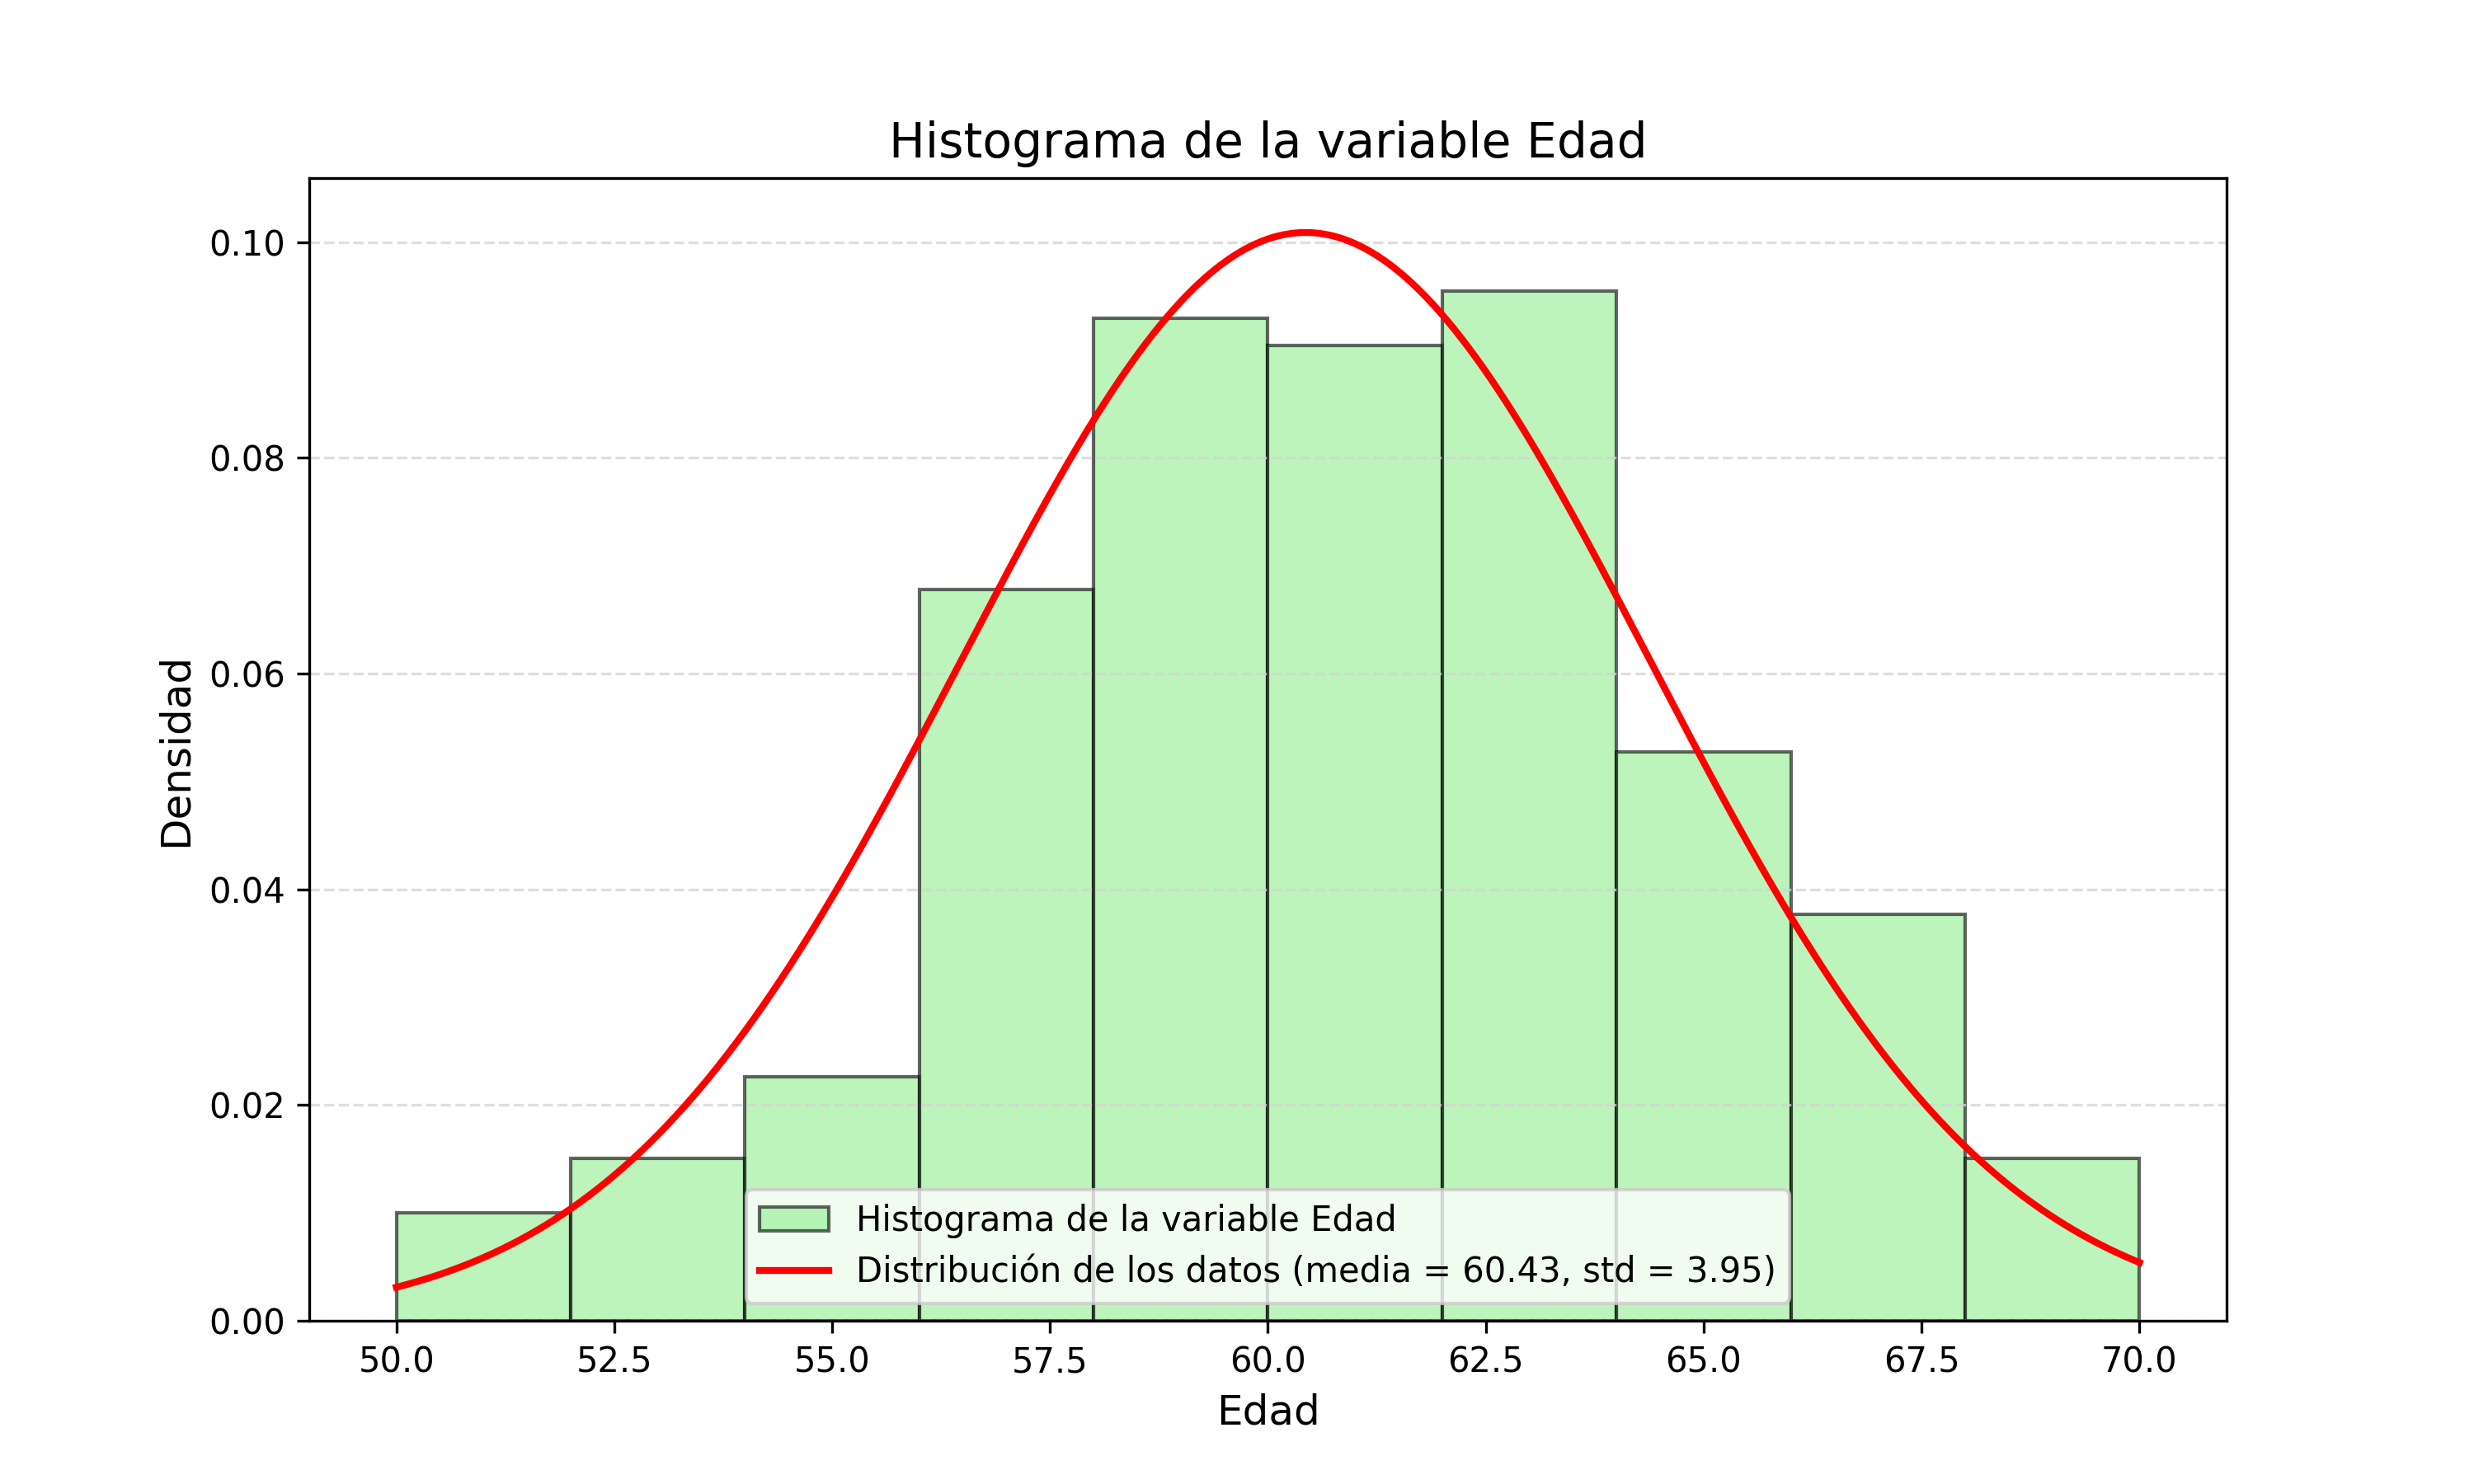
\includegraphics[width=1\textwidth]{img/Histogramas/Histograma_Edad.png}
\end{figure}

\vspace {-1cm}
\begin{figure}[H]
    \centering
    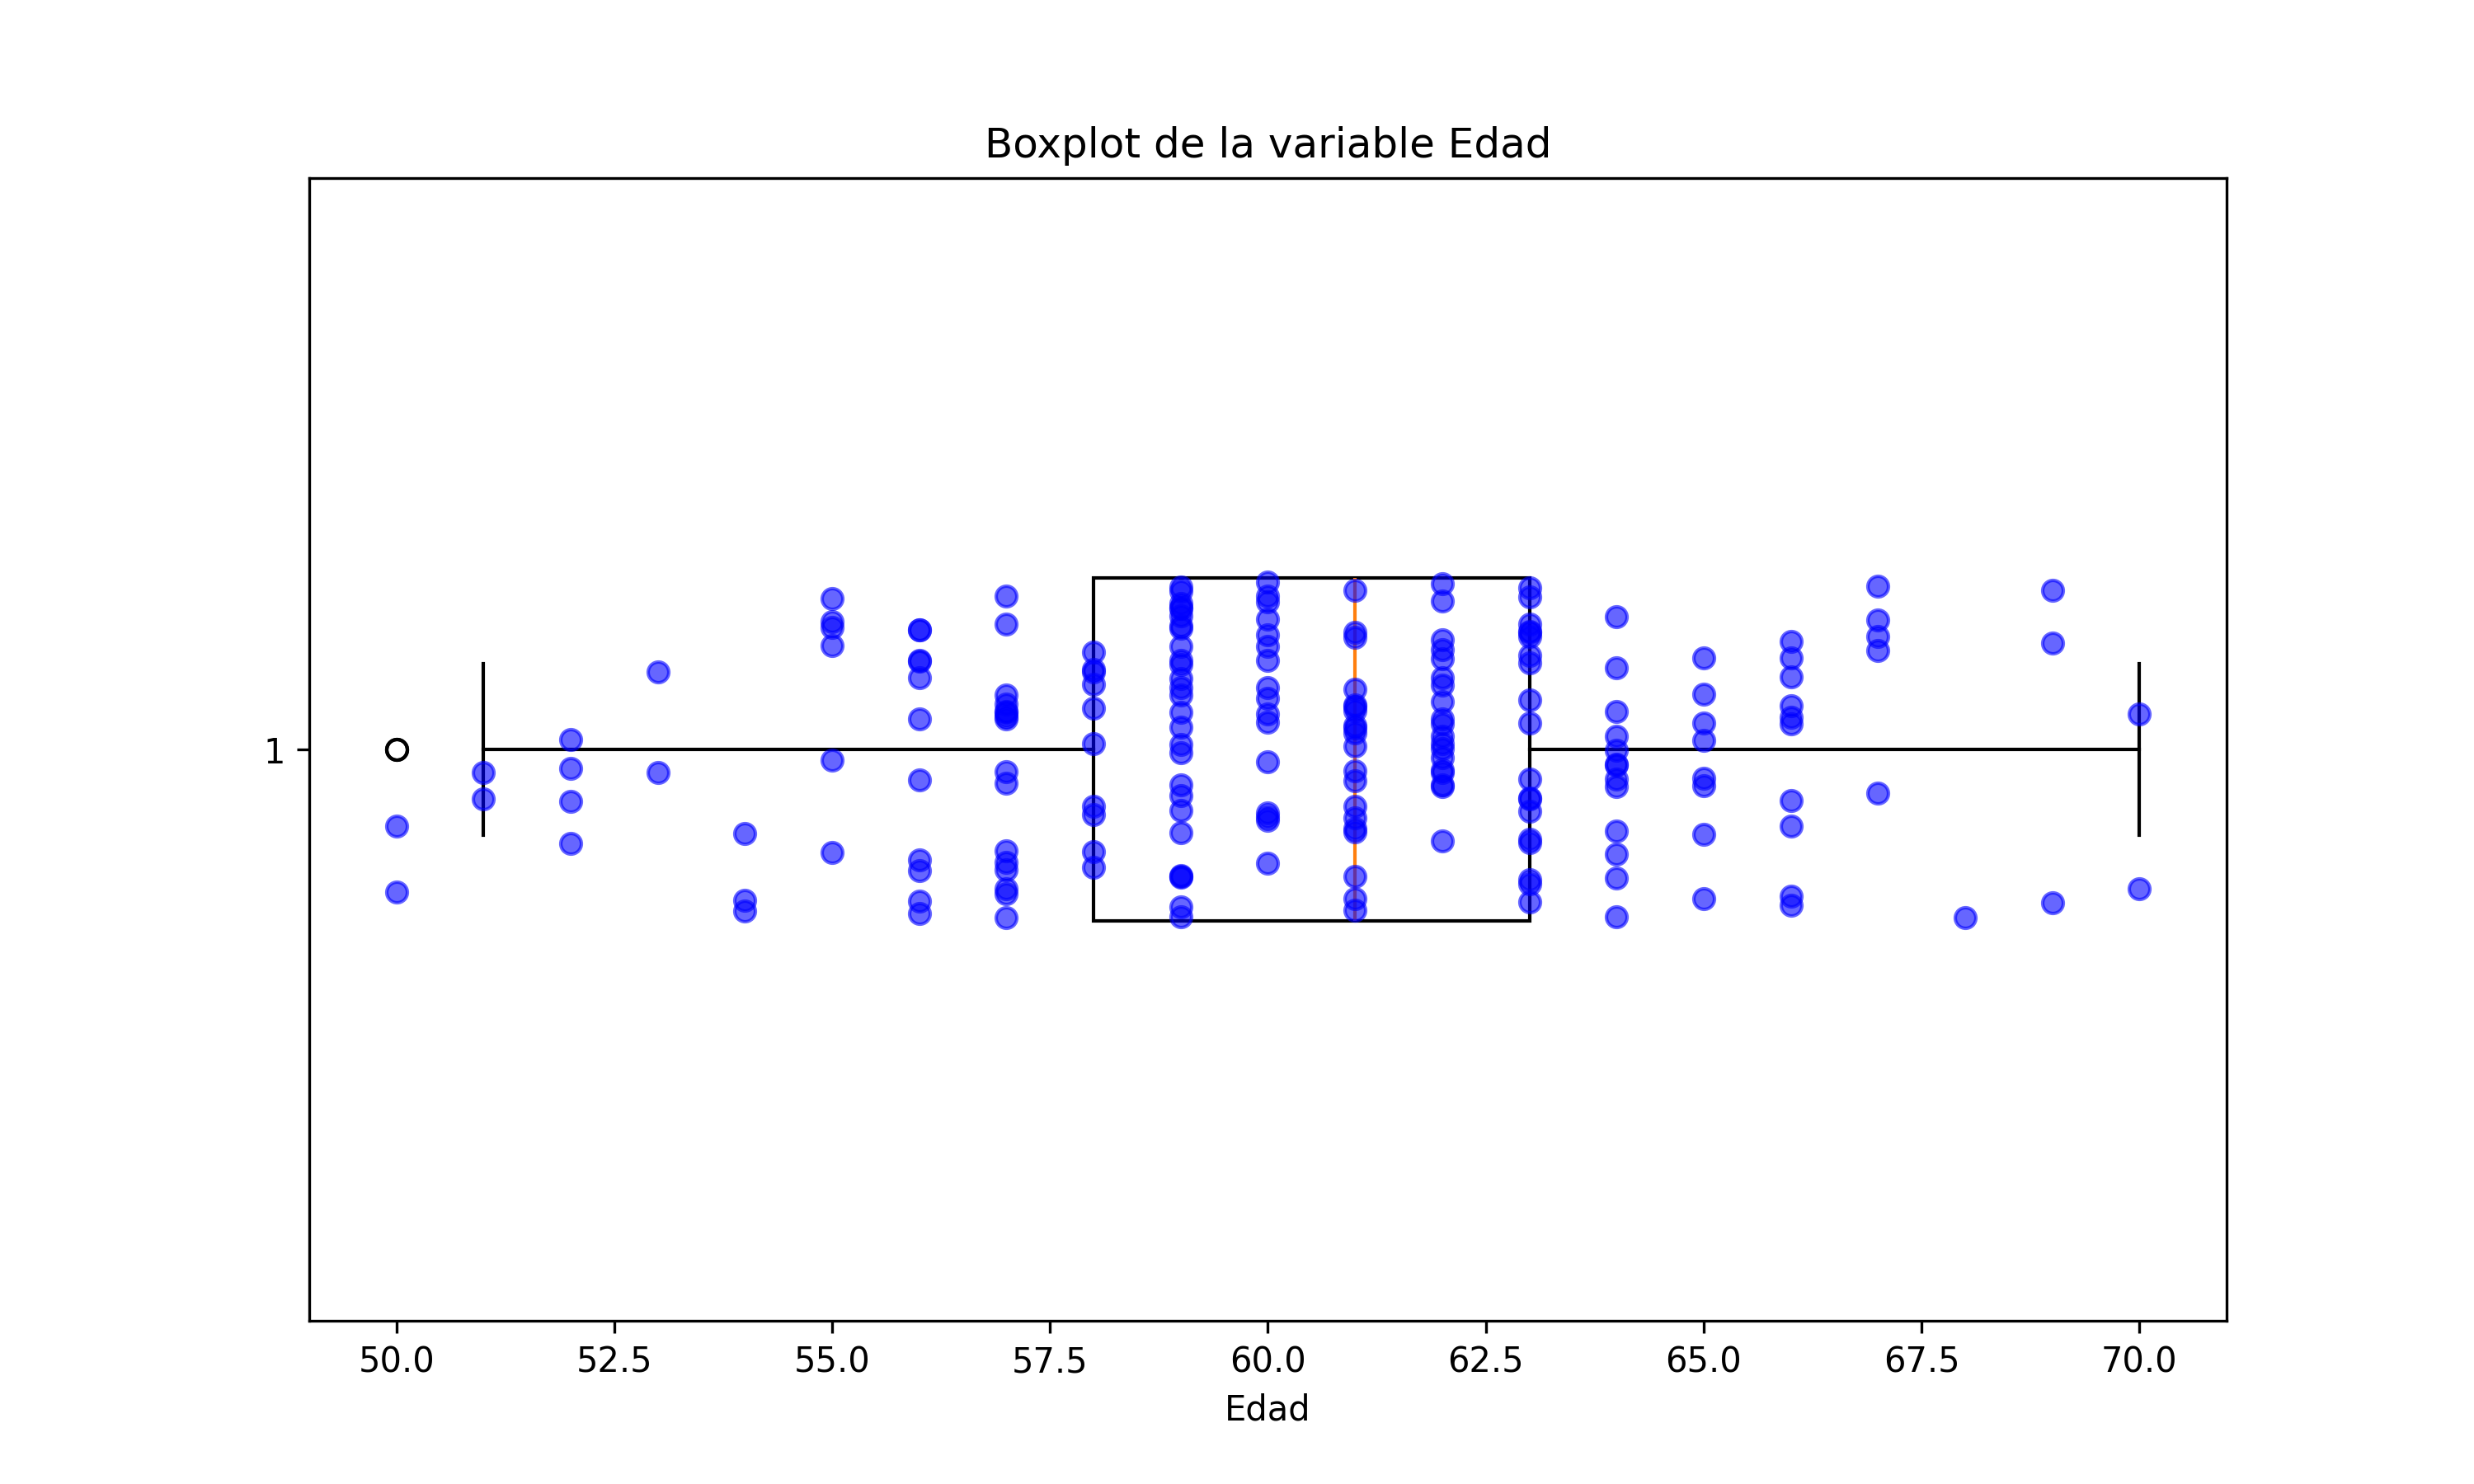
\includegraphics[width=0.9\textwidth]{img/Boxplot/Boxplt_Edad.png}
\end{figure}

\begin{figure}[H]
    \centering
    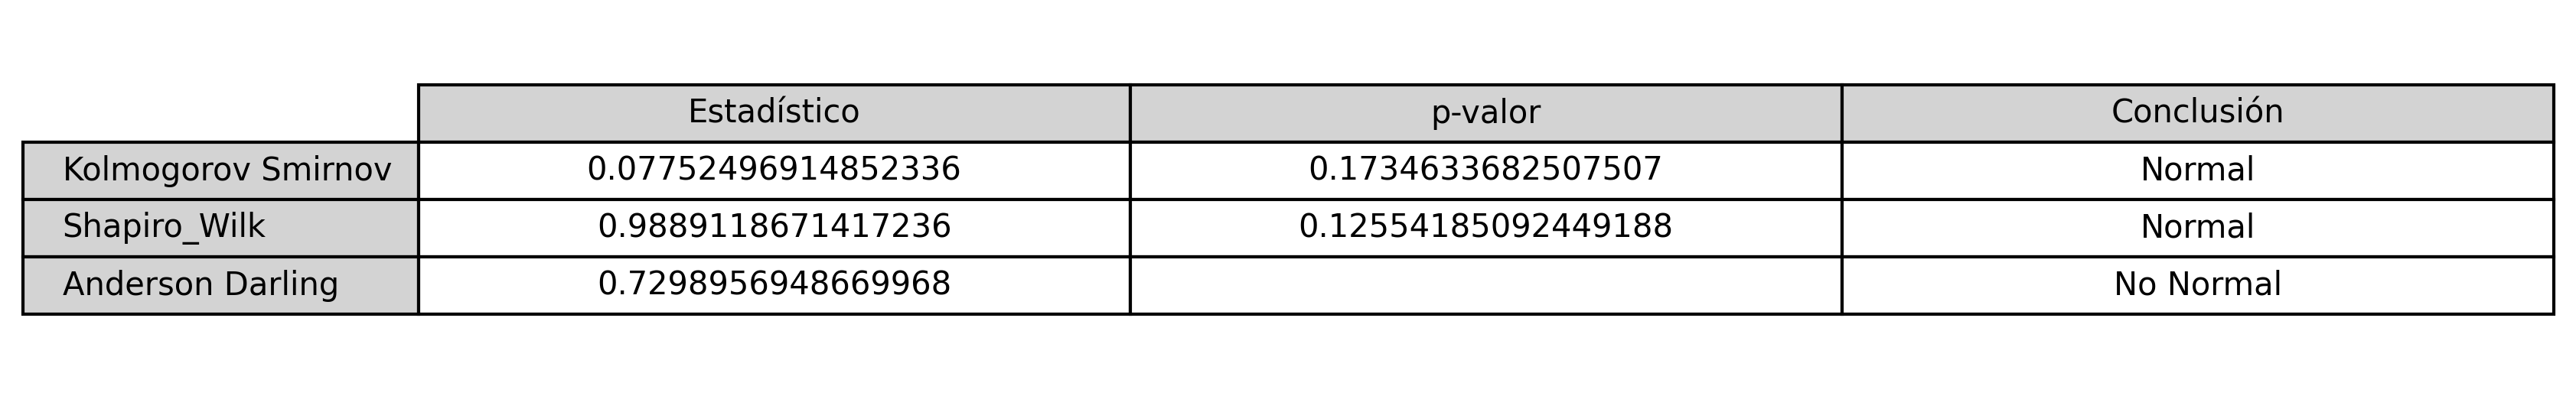
\includegraphics[width=1\textwidth]{img/Tablas/test_normalidad_Edad.png}
\end{figure}


El histograma y el boxplot de la variable Edad visualiza las conclusiones obtenidas a partir de los estadísticos de centro y 
dispersión. La distribución de esta variable es bastante simétrica, con la mayoría de los individuos concentrados alrededor 
de la media y con una ausencia de valores atípicos significativos. La mayor frecuencia de edades se encuentra entre los 58 y 63 años. Esta distribución uniforme y centrada alrededor de la media 
facilita el análisis y la interpretación de los datos, ya que reduce la influencia de valores extremos. Podemos concluir con los resultados de los test de normalidad.





\section{Distribución de la variable AvgGlucosa}
\begin{figure}[H]
    \centering
    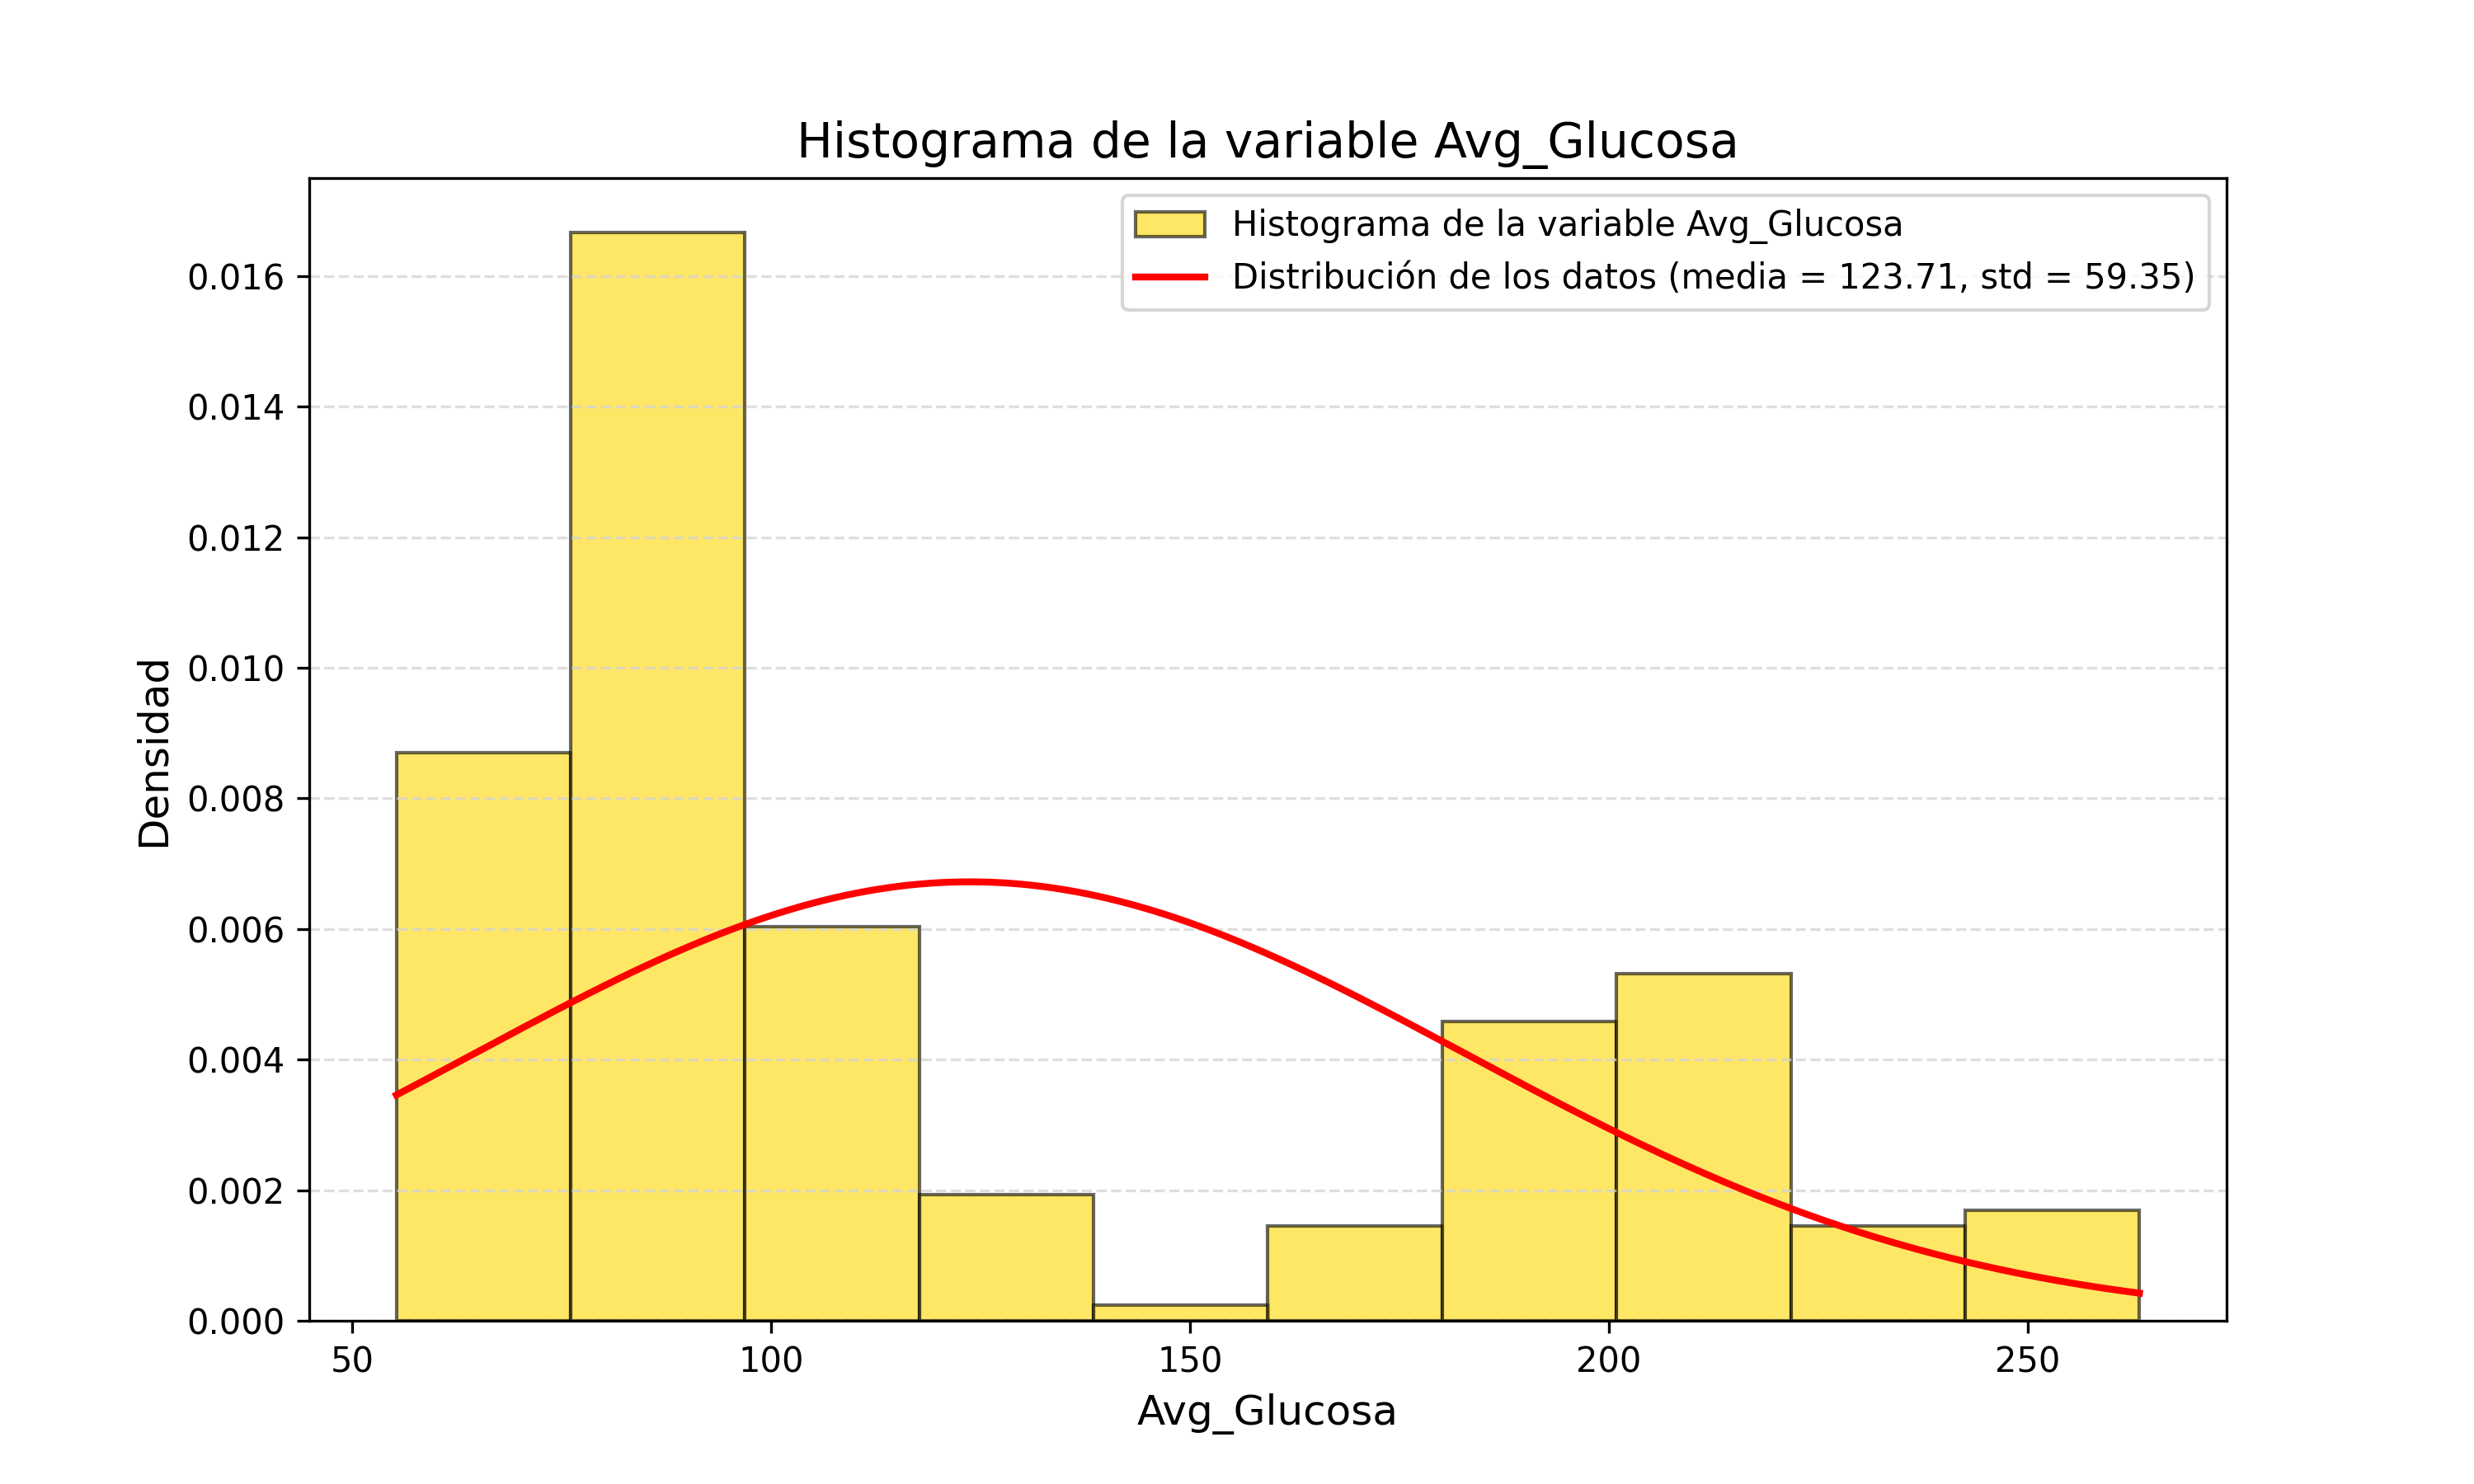
\includegraphics[width=1\textwidth]{img/Histogramas/Histograma_Avg_Glucosa.png}
\end{figure}

\begin{figure}[H]
    \centering
    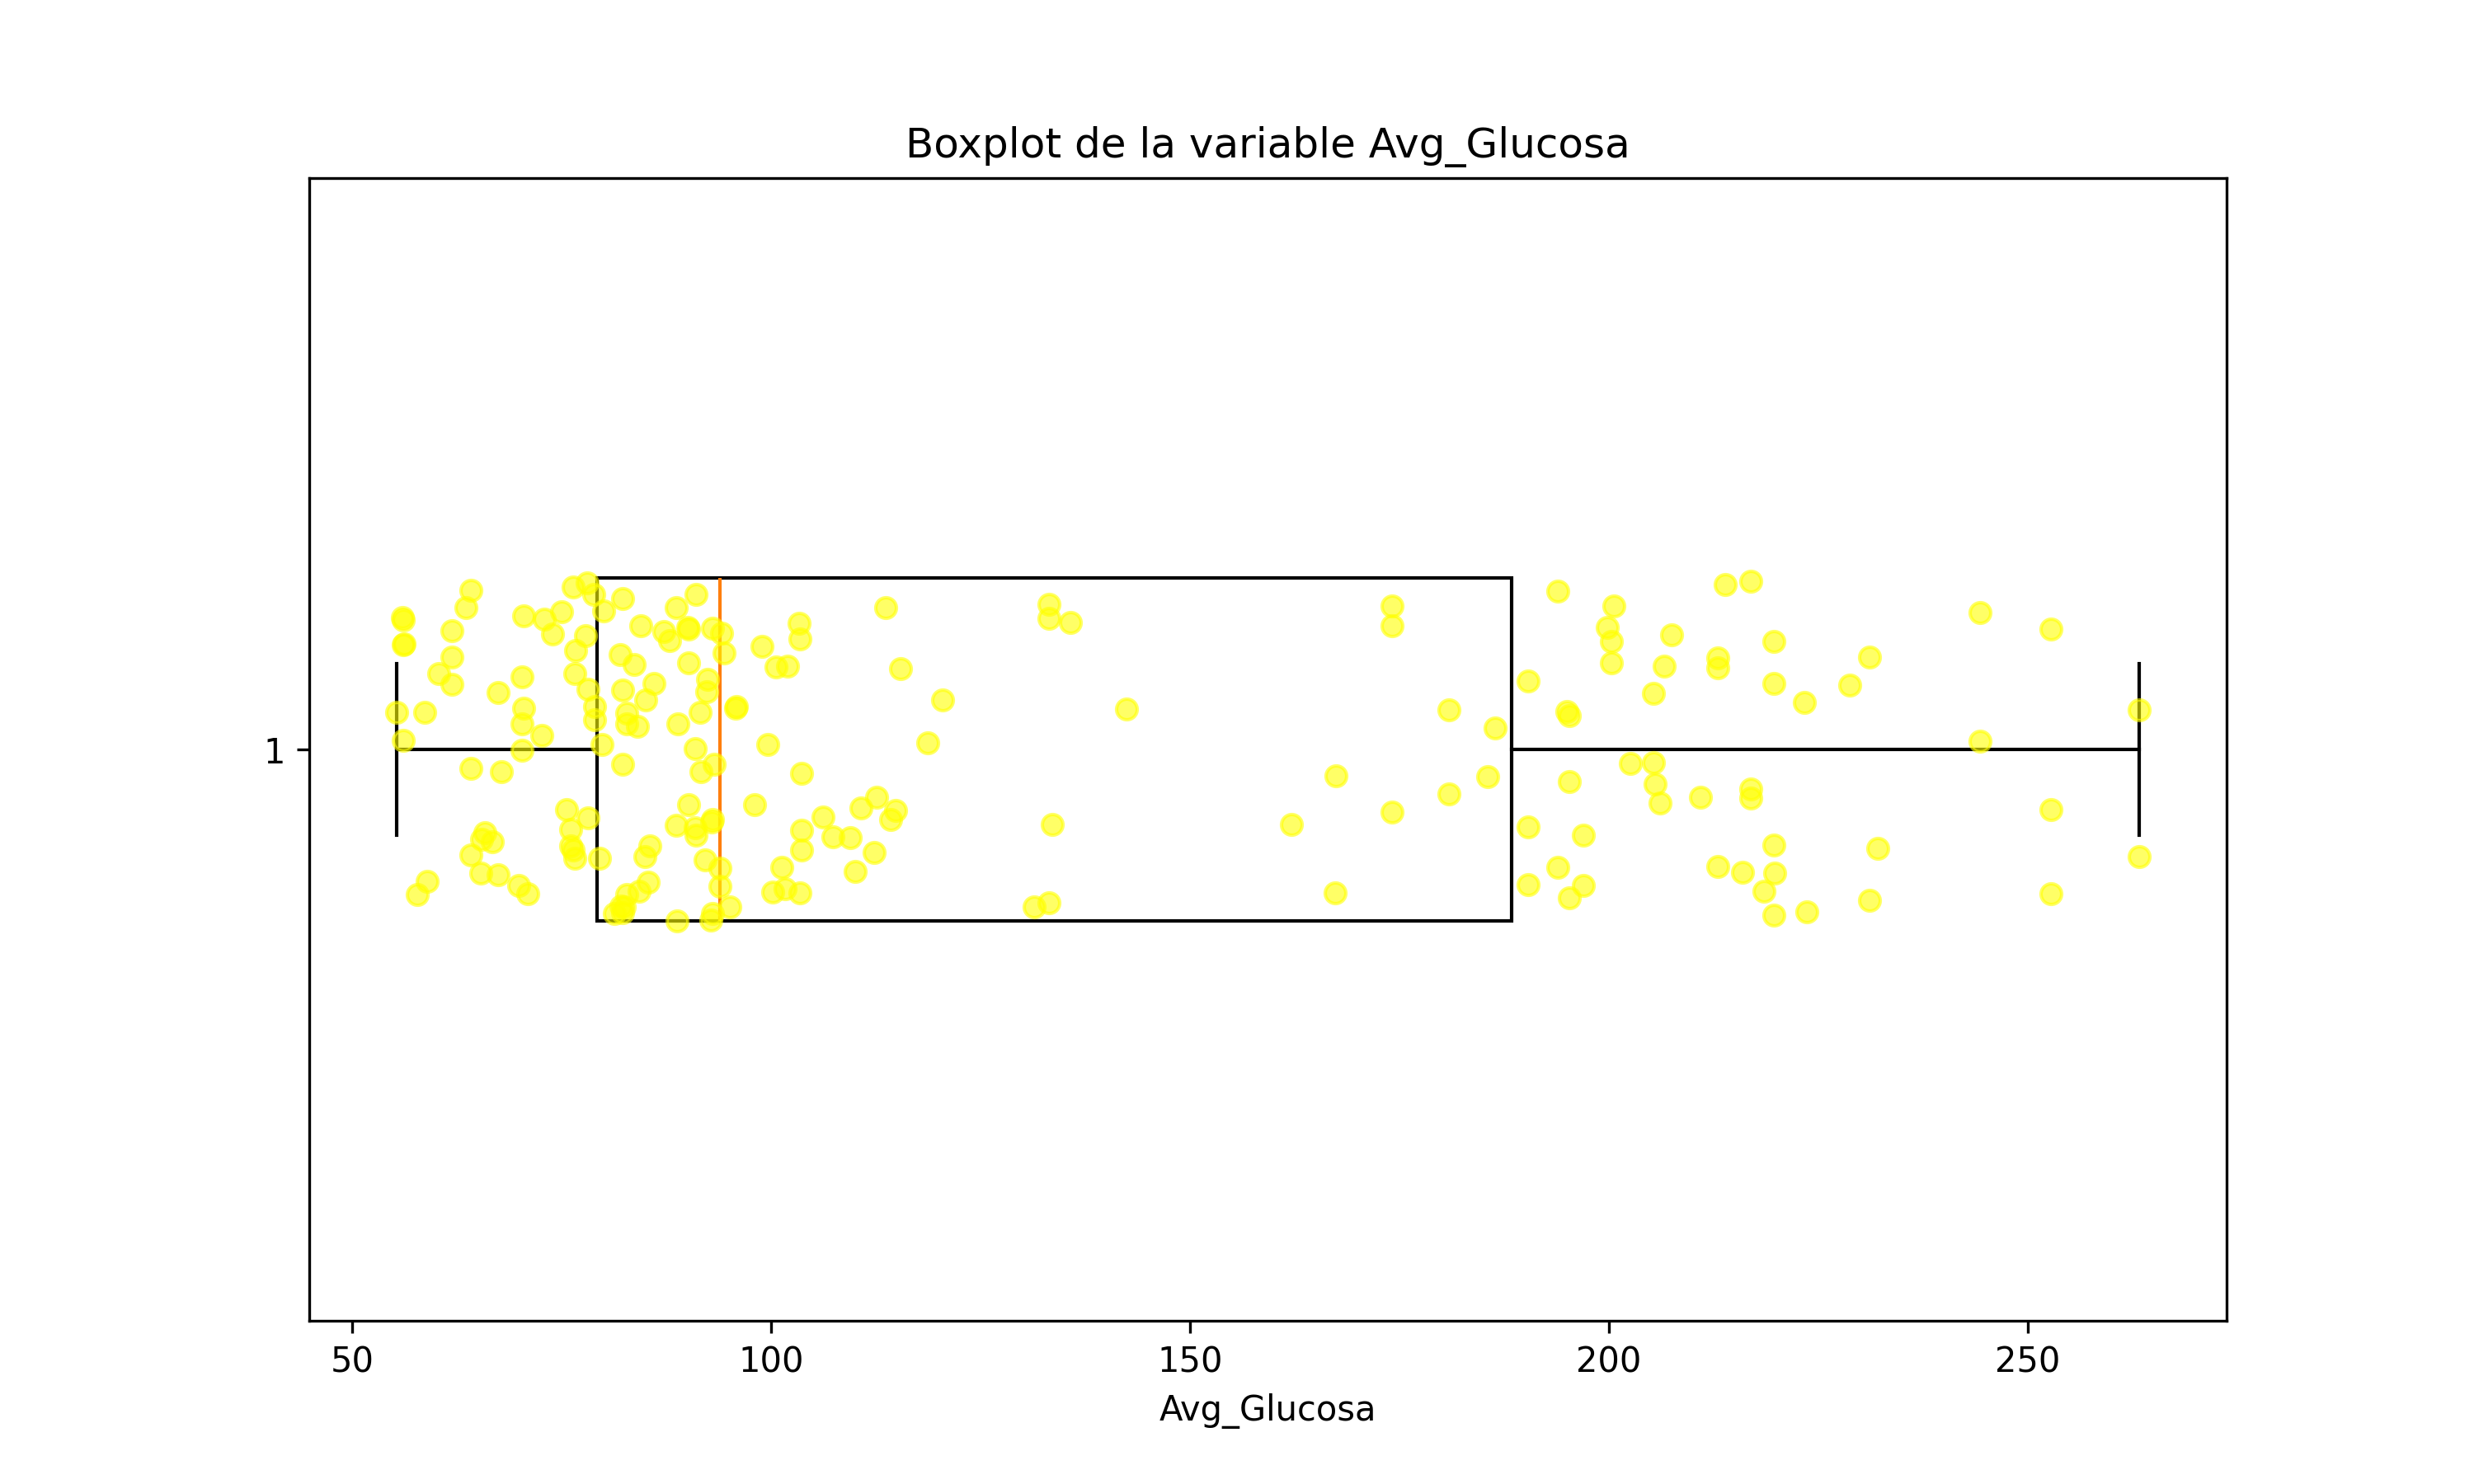
\includegraphics[width=1\textwidth]{img/Boxplot/Boxplt_Avg_Glucosa.png}
\end{figure}

\begin{figure}[H]
    \centering
    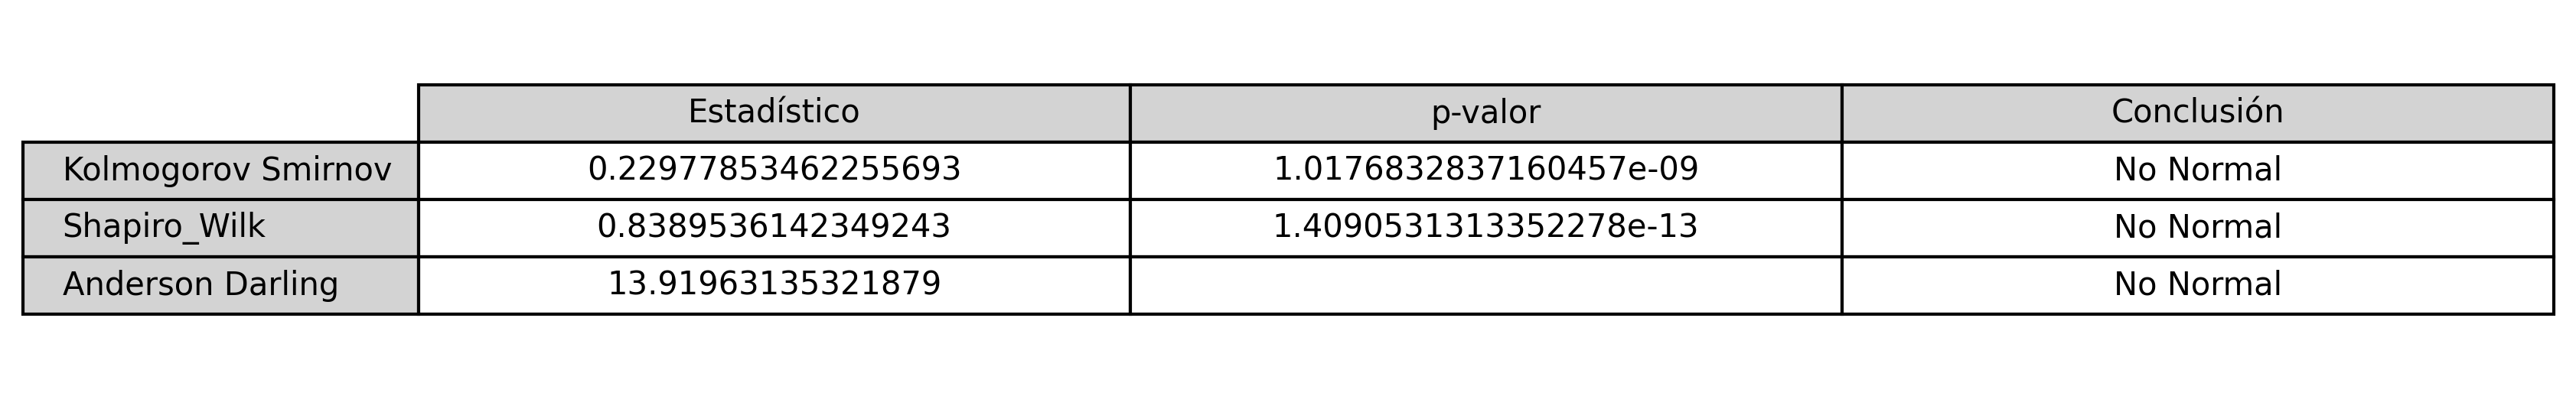
\includegraphics[width=1\textwidth]{img/Tablas/test_normalidad_Avg_Glucosa.png}
\end{figure}

En los gráficos de la variable Nivel Promedio de Glucosa en Sangre, se aprecia una concentración de observaciones en el intervalo de 60 a 100, podemos observar en el boxplot como la caja se encuentra inquinada a la parte izquierda del plano.
Es evidente la asimetría en esta distribución con notables valores atípicos extremos.



\section{Distribución de la variable IMC}

\begin{figure}[H]
    \centering
    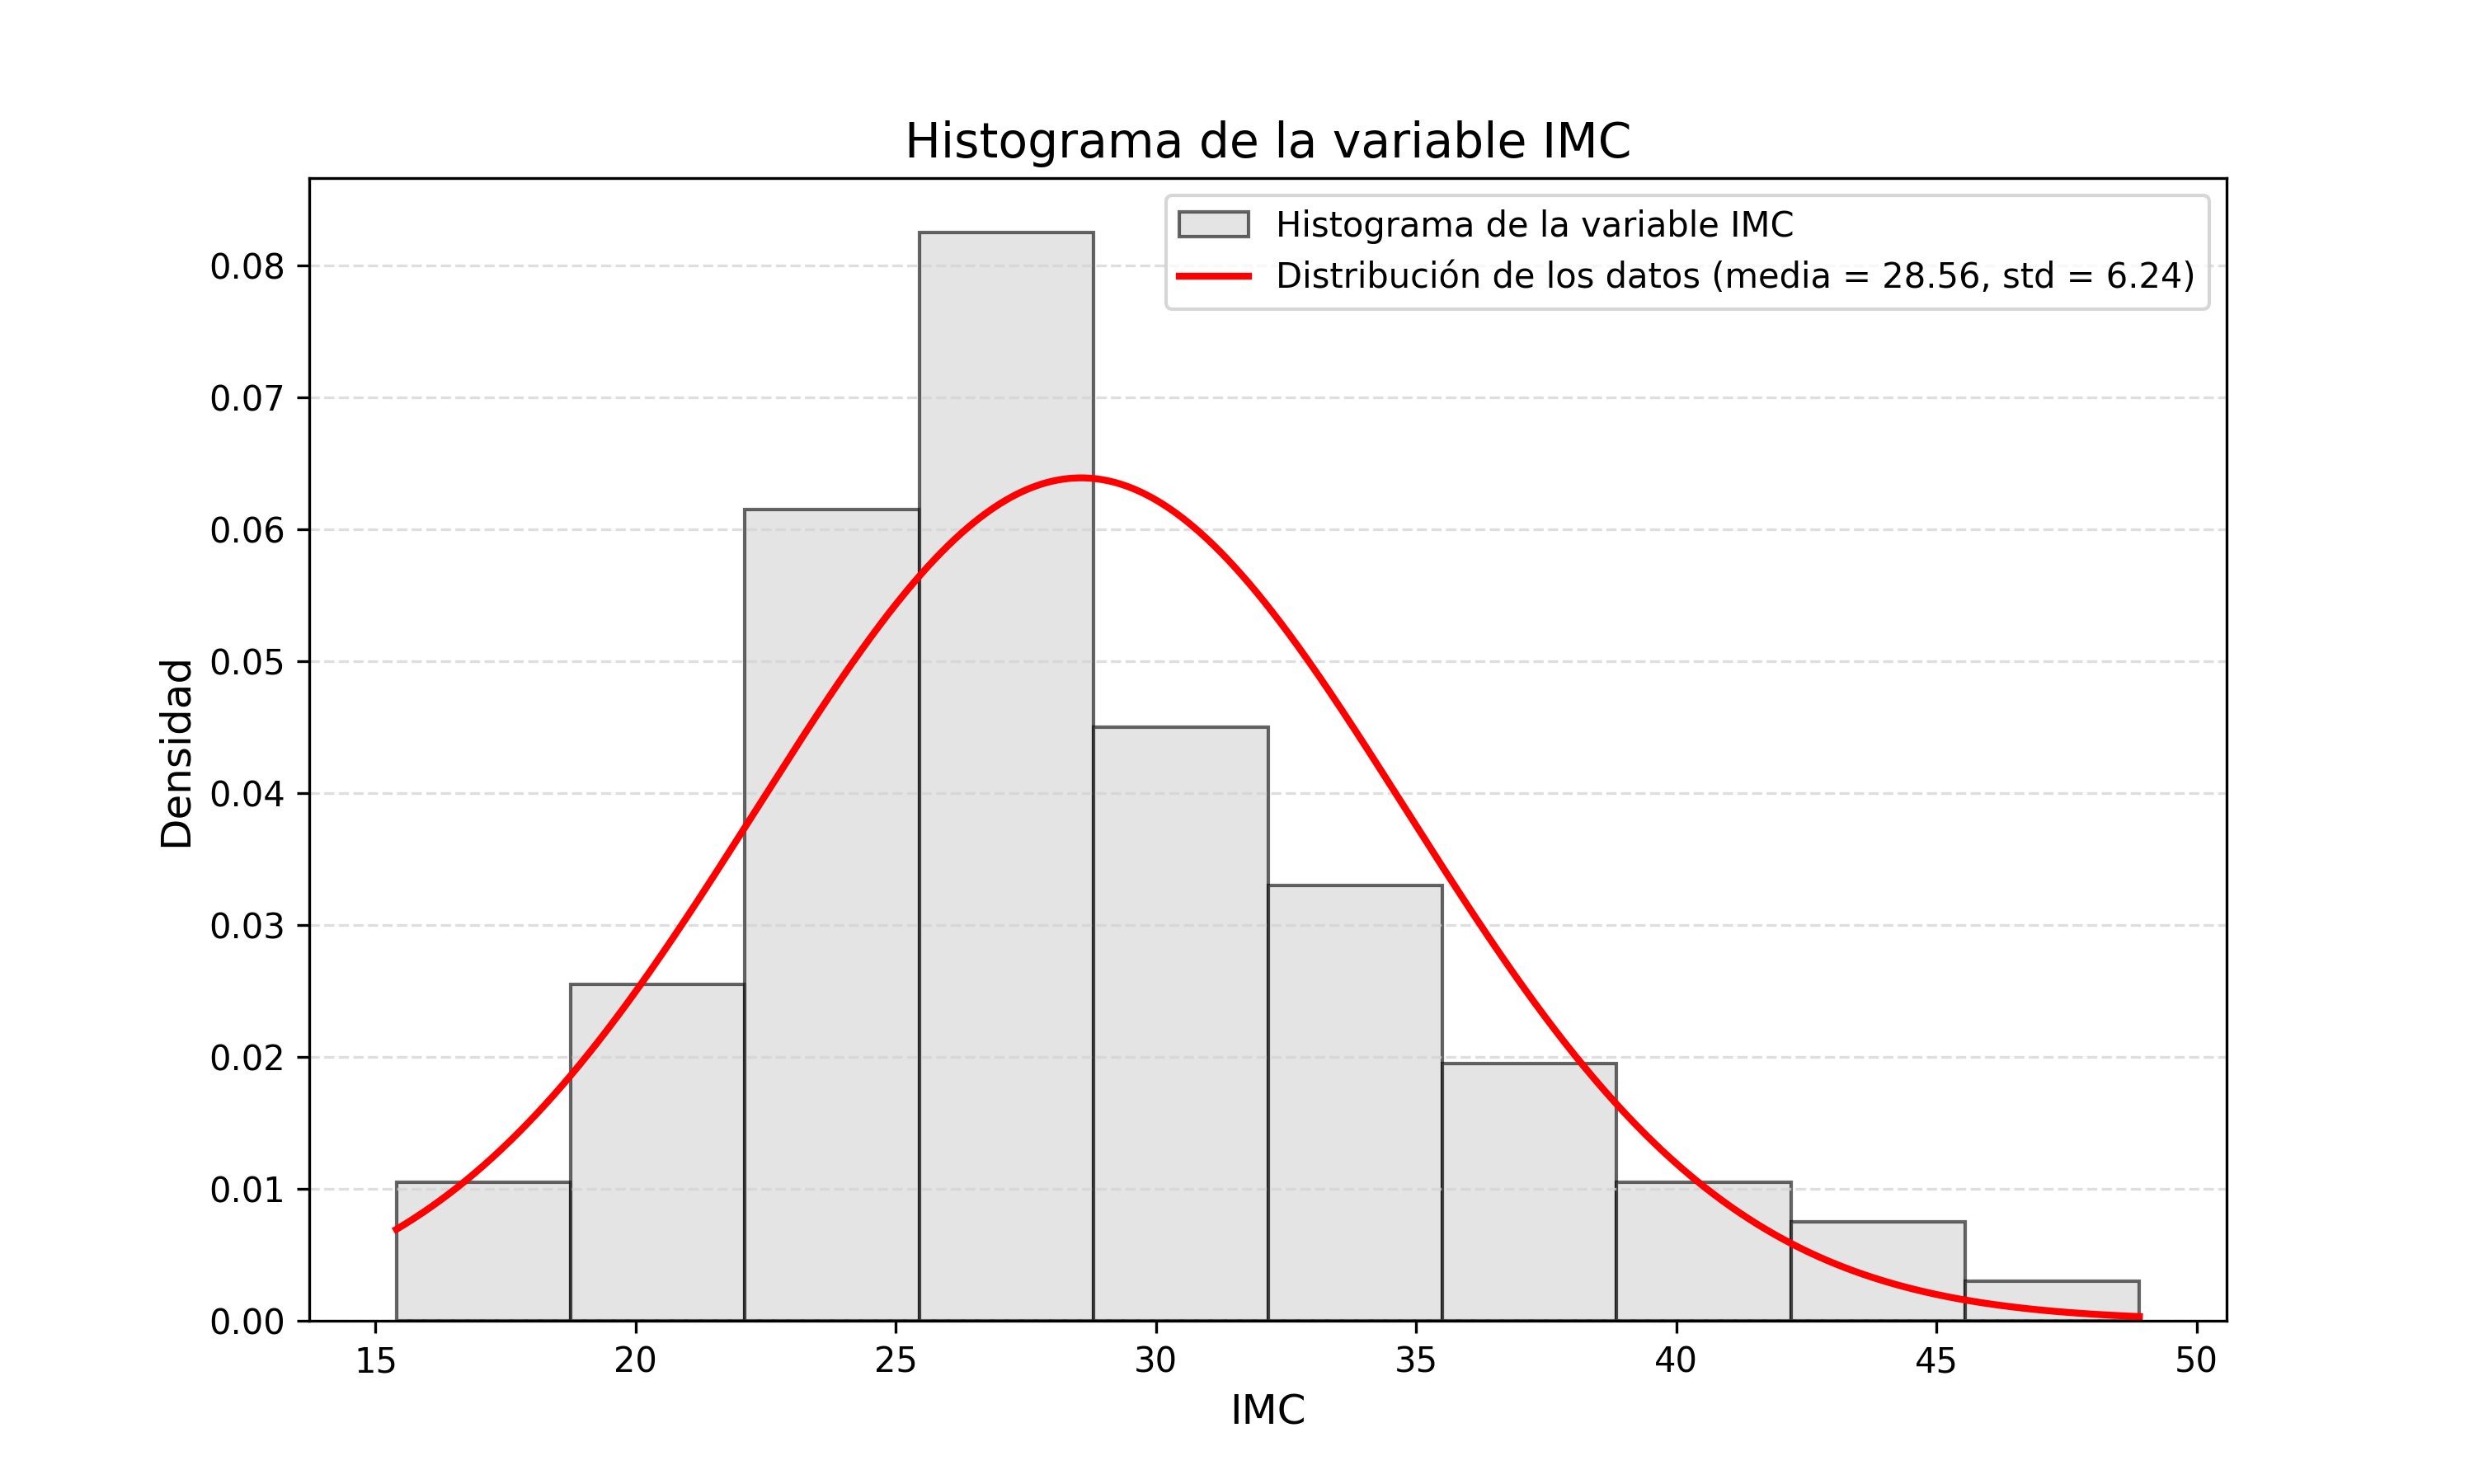
\includegraphics[width=1\textwidth]{img/Histogramas/Histograma_IMC.png}
\end{figure}

\begin{figure}[H]
    \centering
    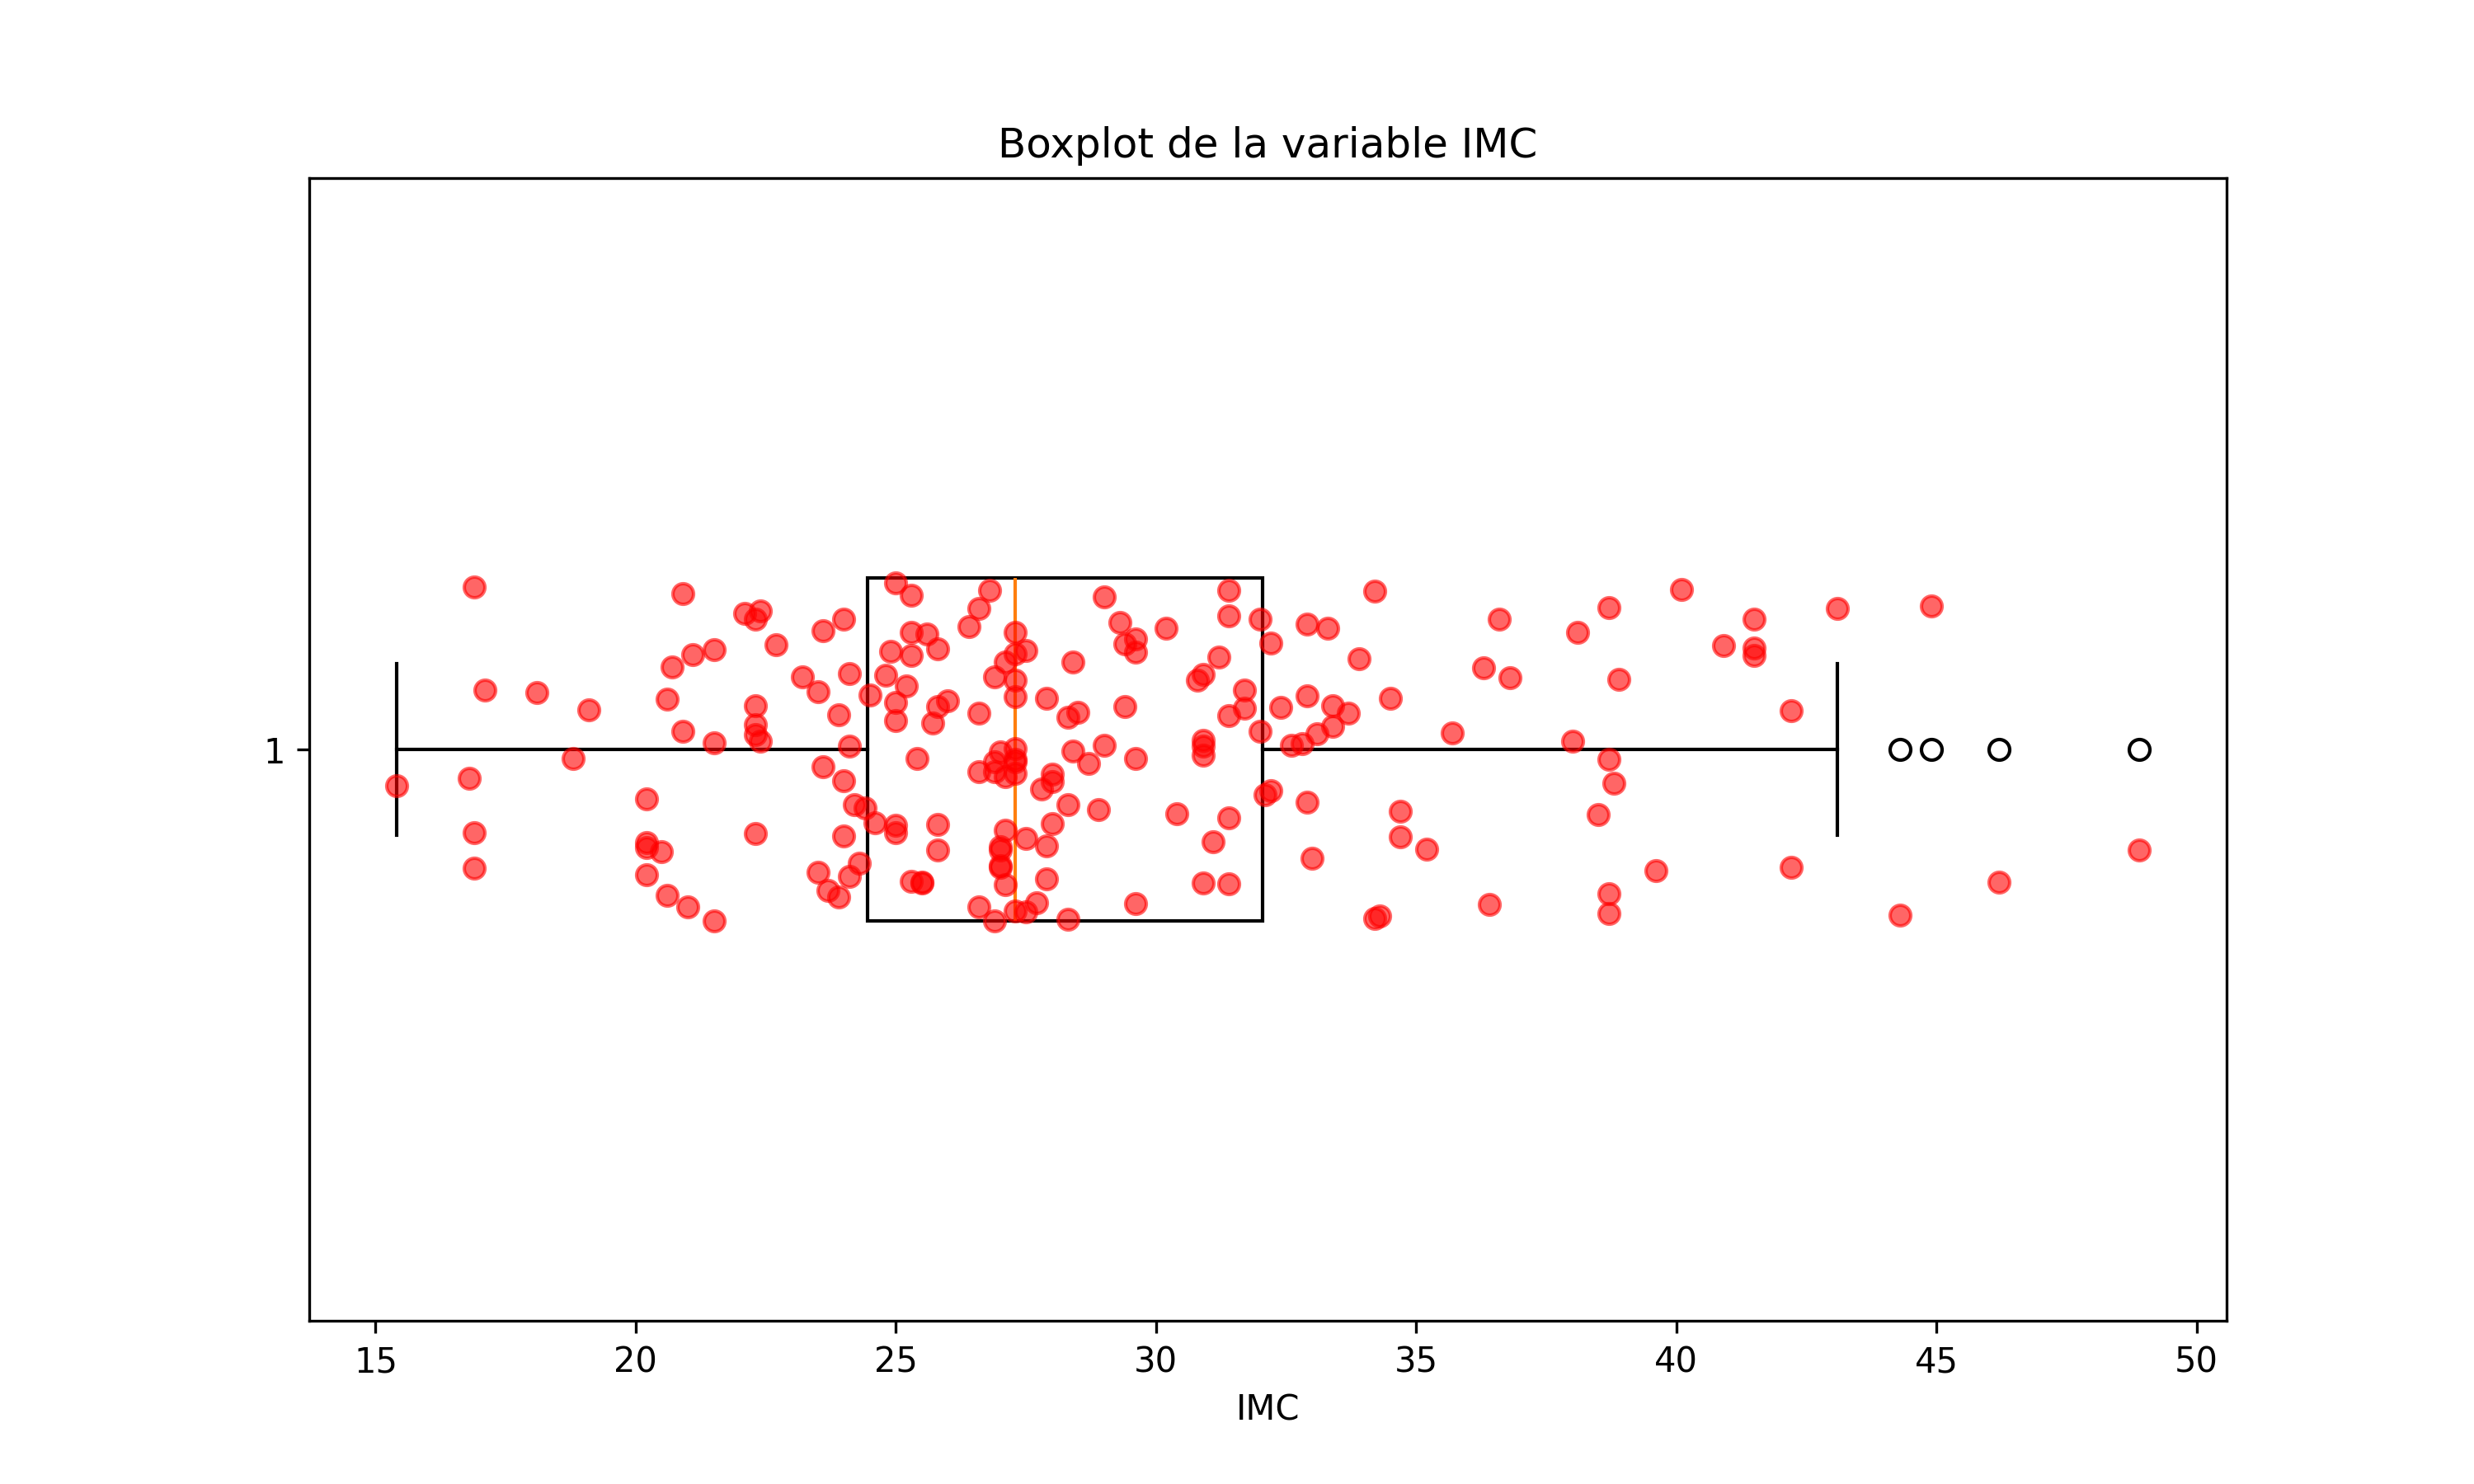
\includegraphics[width=1\textwidth]{img/Boxplot/Boxplt_IMC.png}
\end{figure}

\begin{figure}[H]
    \centering
    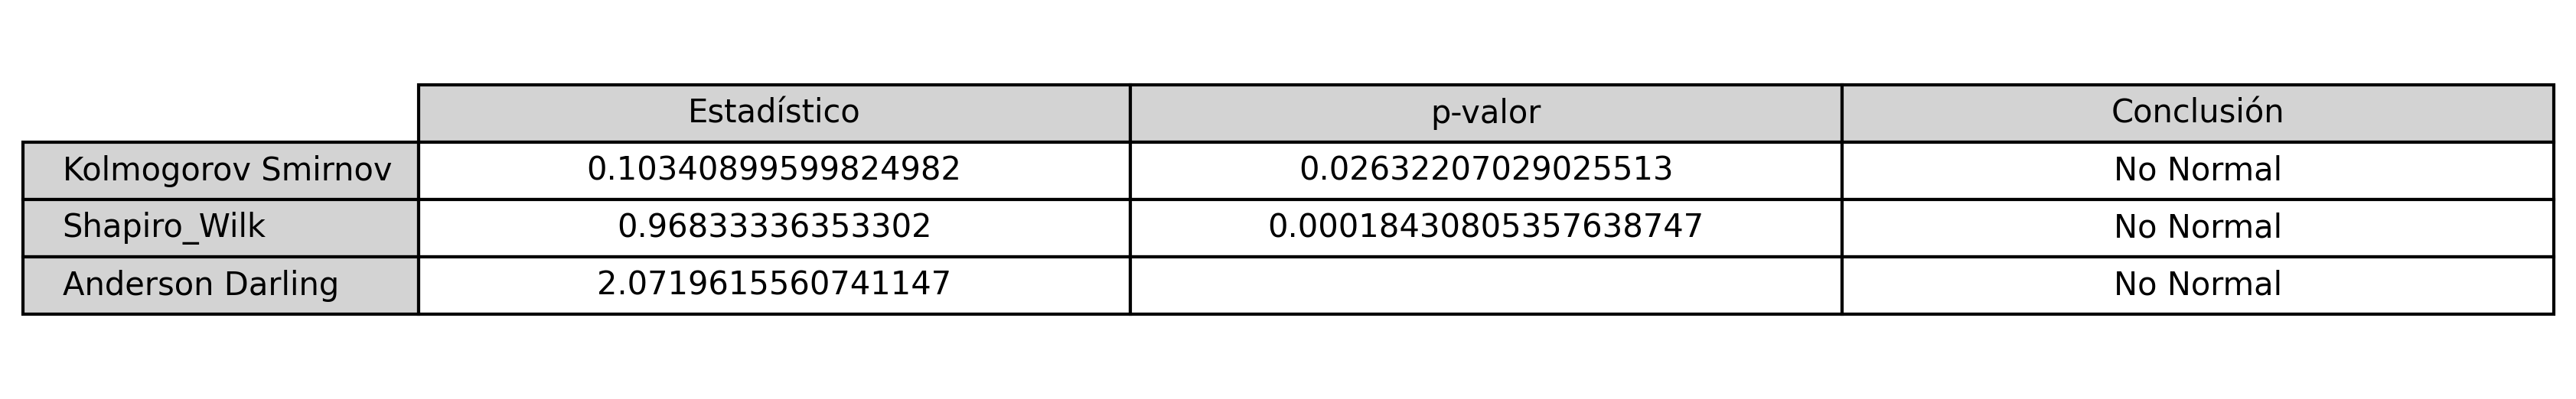
\includegraphics[width=1\textwidth]{img/Tablas/test_normalidad_IMC.png}
\end{figure}


En estos gráficos de la variable Índice de Masa Corporal (IMC) se observan en el intervalo de 40 a 50 kg/m\^2 valores extremos en 
la variable que distorsionan la uniformidad de su distribución corroborando los valores de las medidas de dispersión de esta variable. 
También se observa que hay un grupo grande de individuos con un índice de masa corporal entre los 25 y 30 kg/m\^2. Con los resultados 
de los test de normalidad concluimos que esta variable no sigue una distribución normal.









\newpage


\section{Relación entre variables}

\subsection{Matrices de correlacion}
Para visualizar de manera clara la relación entre todas las variables del dataset, utilizamos matrices de correlación. Estas matrices muestran un coeficiente que varía entre -1 y 1 (1: Correlación positiva perfecta, -1: Correlación negativa perfecta, 0: No hay correlación lineal.), el cual mide la fuerza y la dirección de la relación entre las variables. Este análisis es fundamental para determinar modelos de predicción de una variable en función de otras.
\begin{figure}[h]
    \centering
    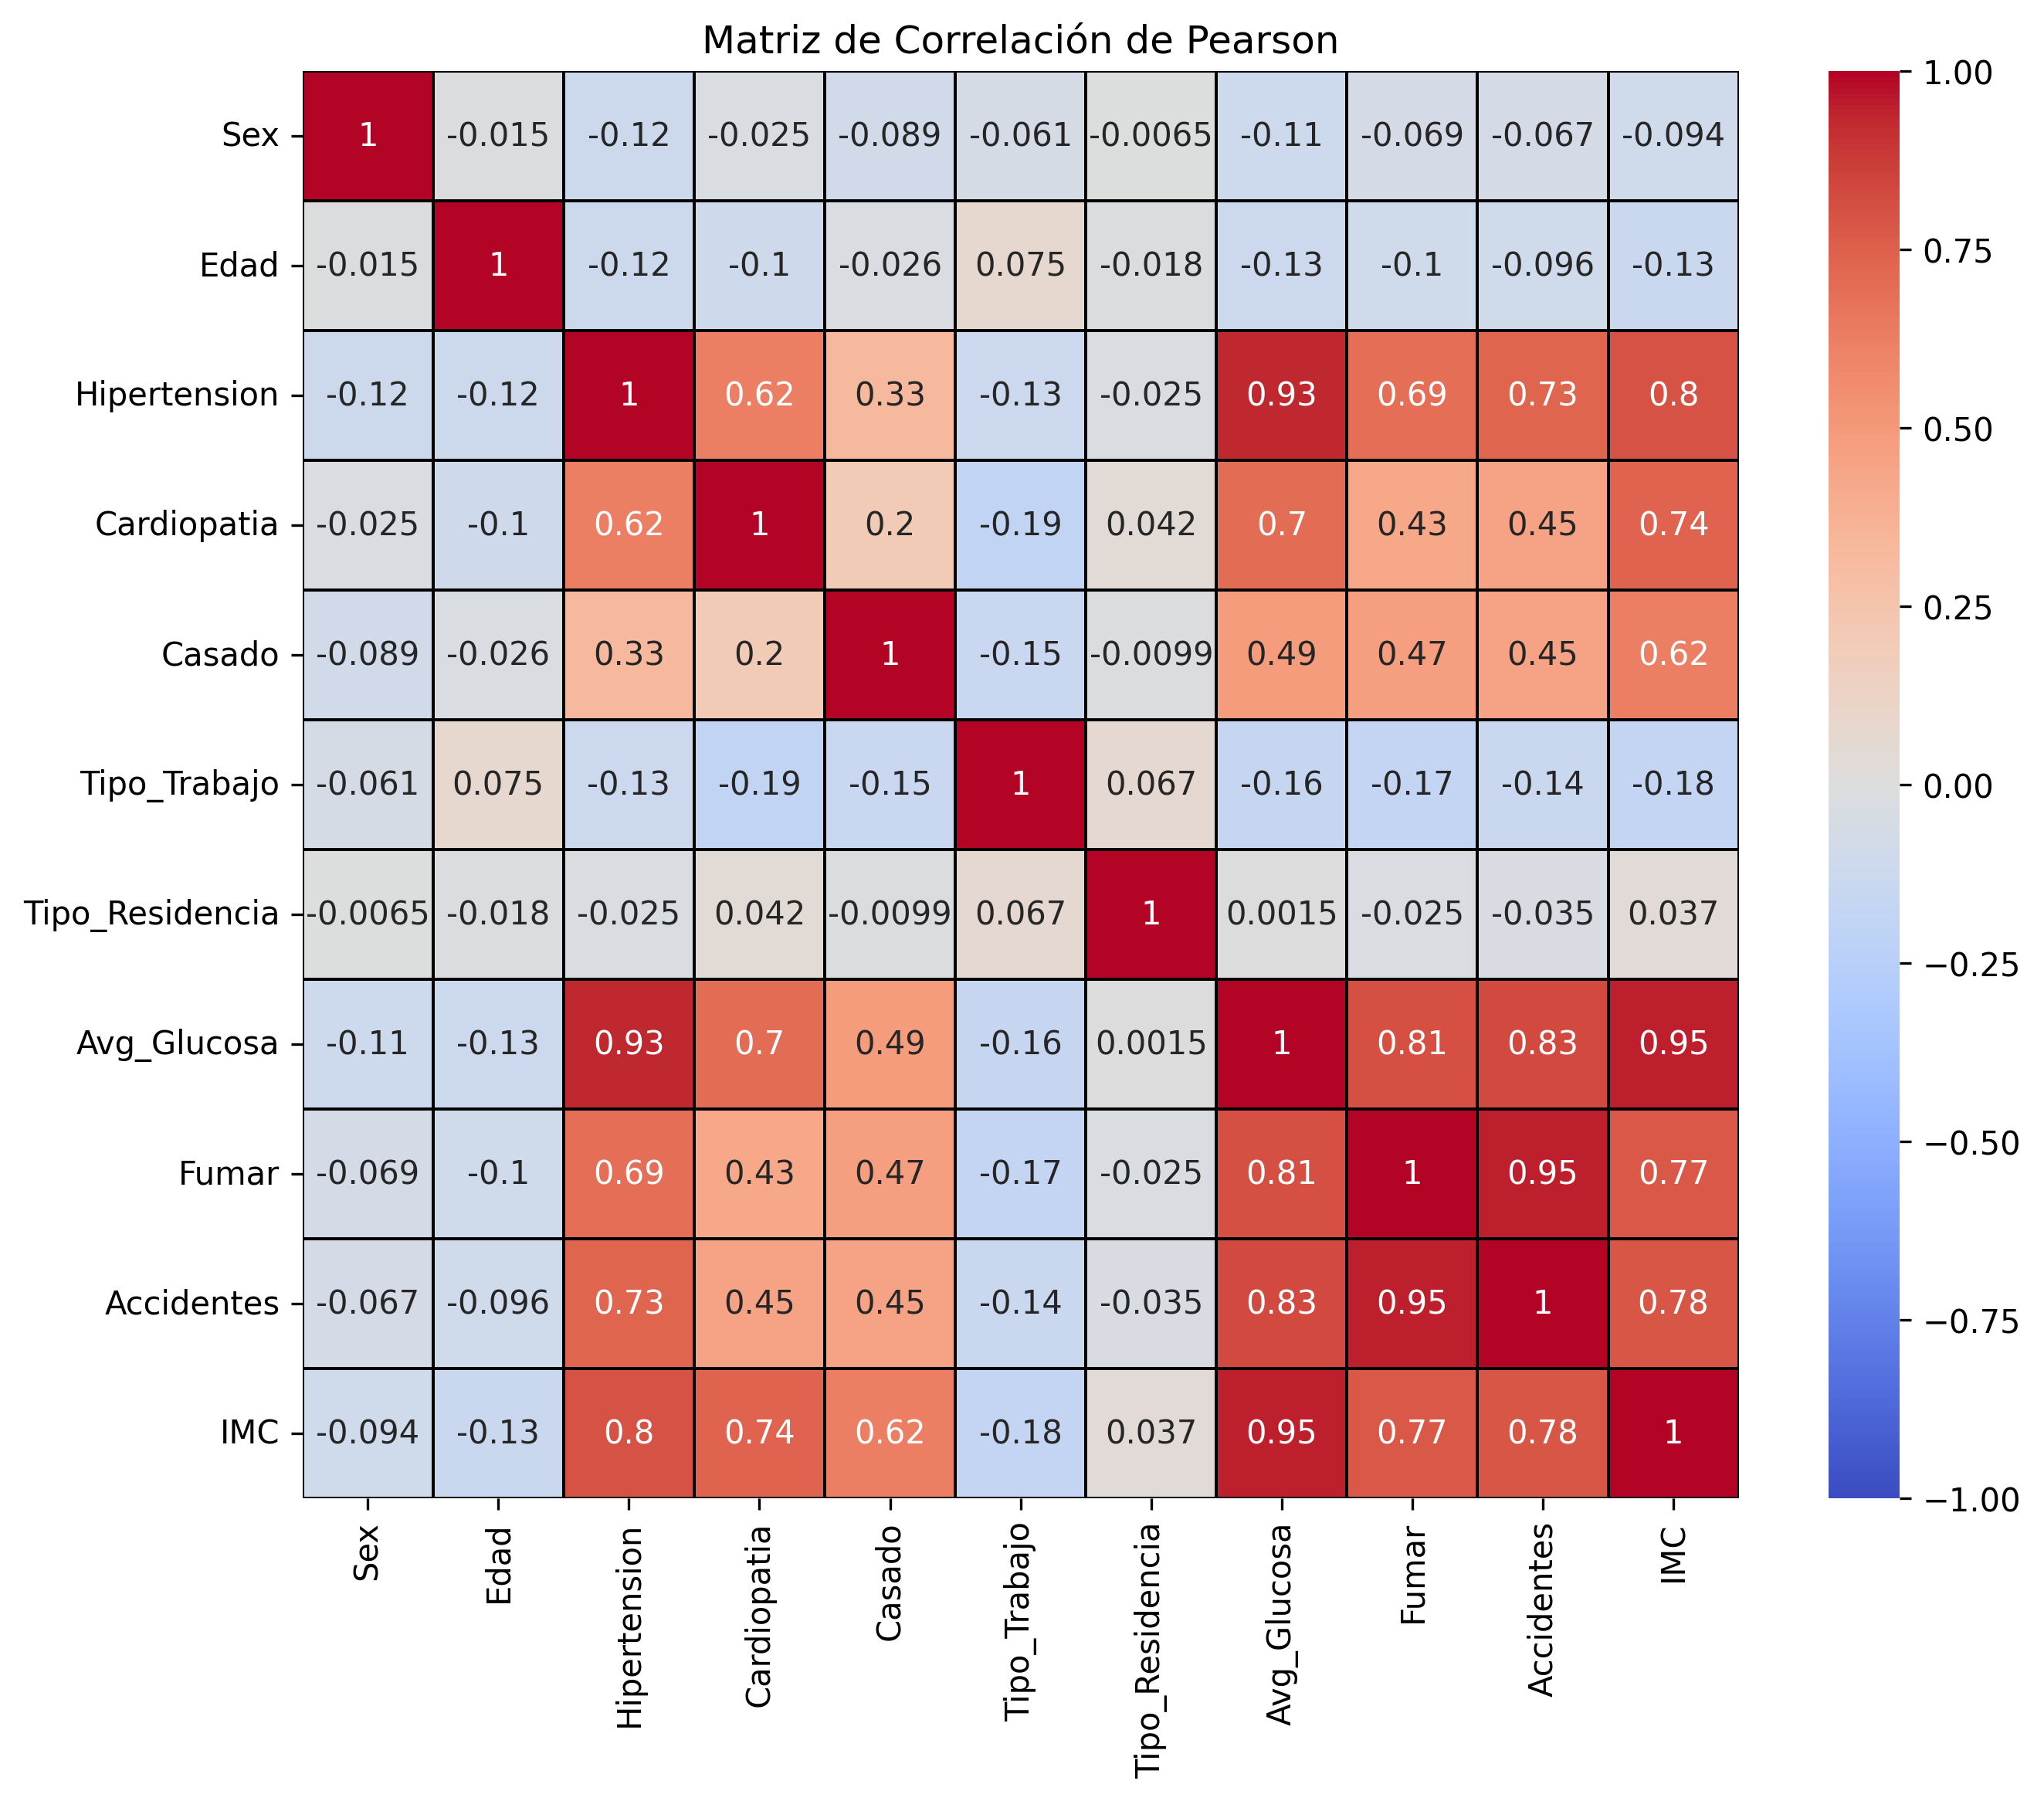
\includegraphics[width=0.9\textwidth]{img/matriz_correlacion_pearson.png}
\end{figure}

El coeficiente de correlación de Pearson mide la relación lineal entre dos variables. En esta matriz, 
observamos que no existen fuertes correlaciones lineales negativas entre las variables. Muchas de ellas 
no presentan correlación significativa, mientras que una cantidad considerable muestra una notable 
correlación positiva por lo que la regresión lineal puede ser un buen modelo para el análisis predictivo de estas últimas.

\begin{figure}[h]
    \centering
    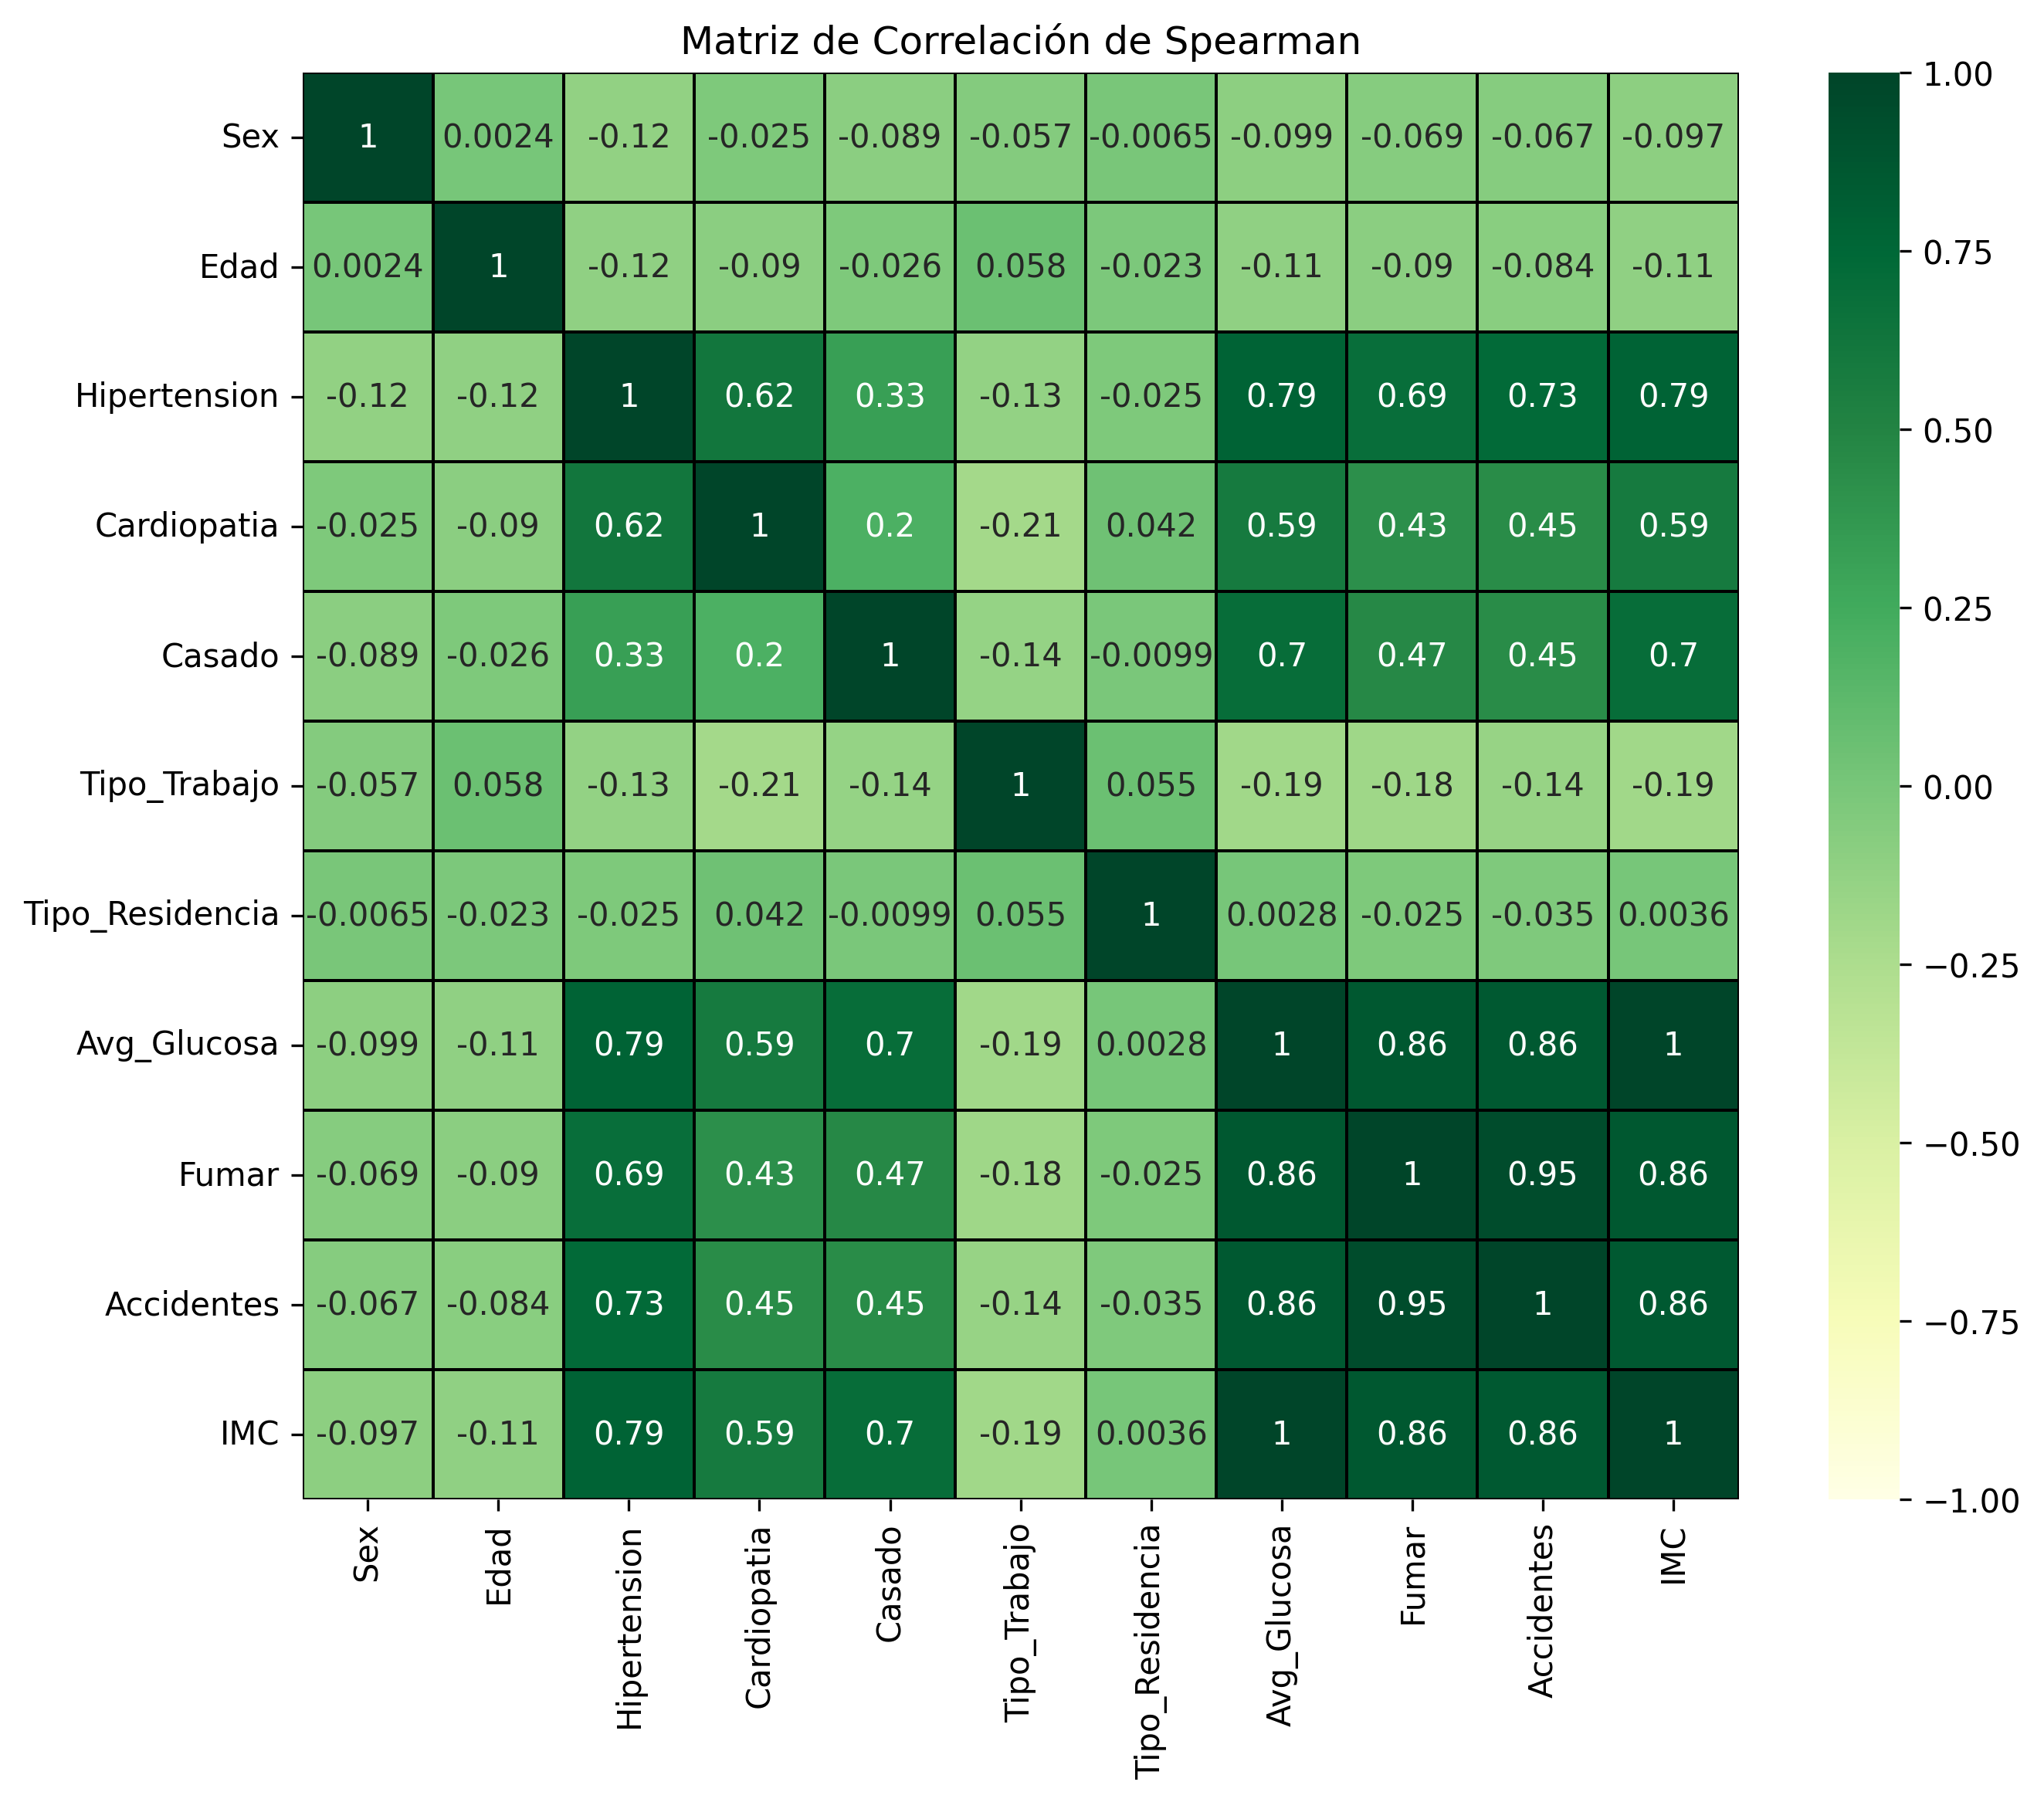
\includegraphics[width=0.9\textwidth]{img/matriz_correlacion_spearman.png}
\end{figure}

Podemos apreciar que la matriz de correlación de Spearman tiene gran similitud con la de Pearson, lo que indica que no tenemos relaciones monotónicas no lineales.


\subsection{Regresión lineal}

\begin{figure}[h]
    \centering
    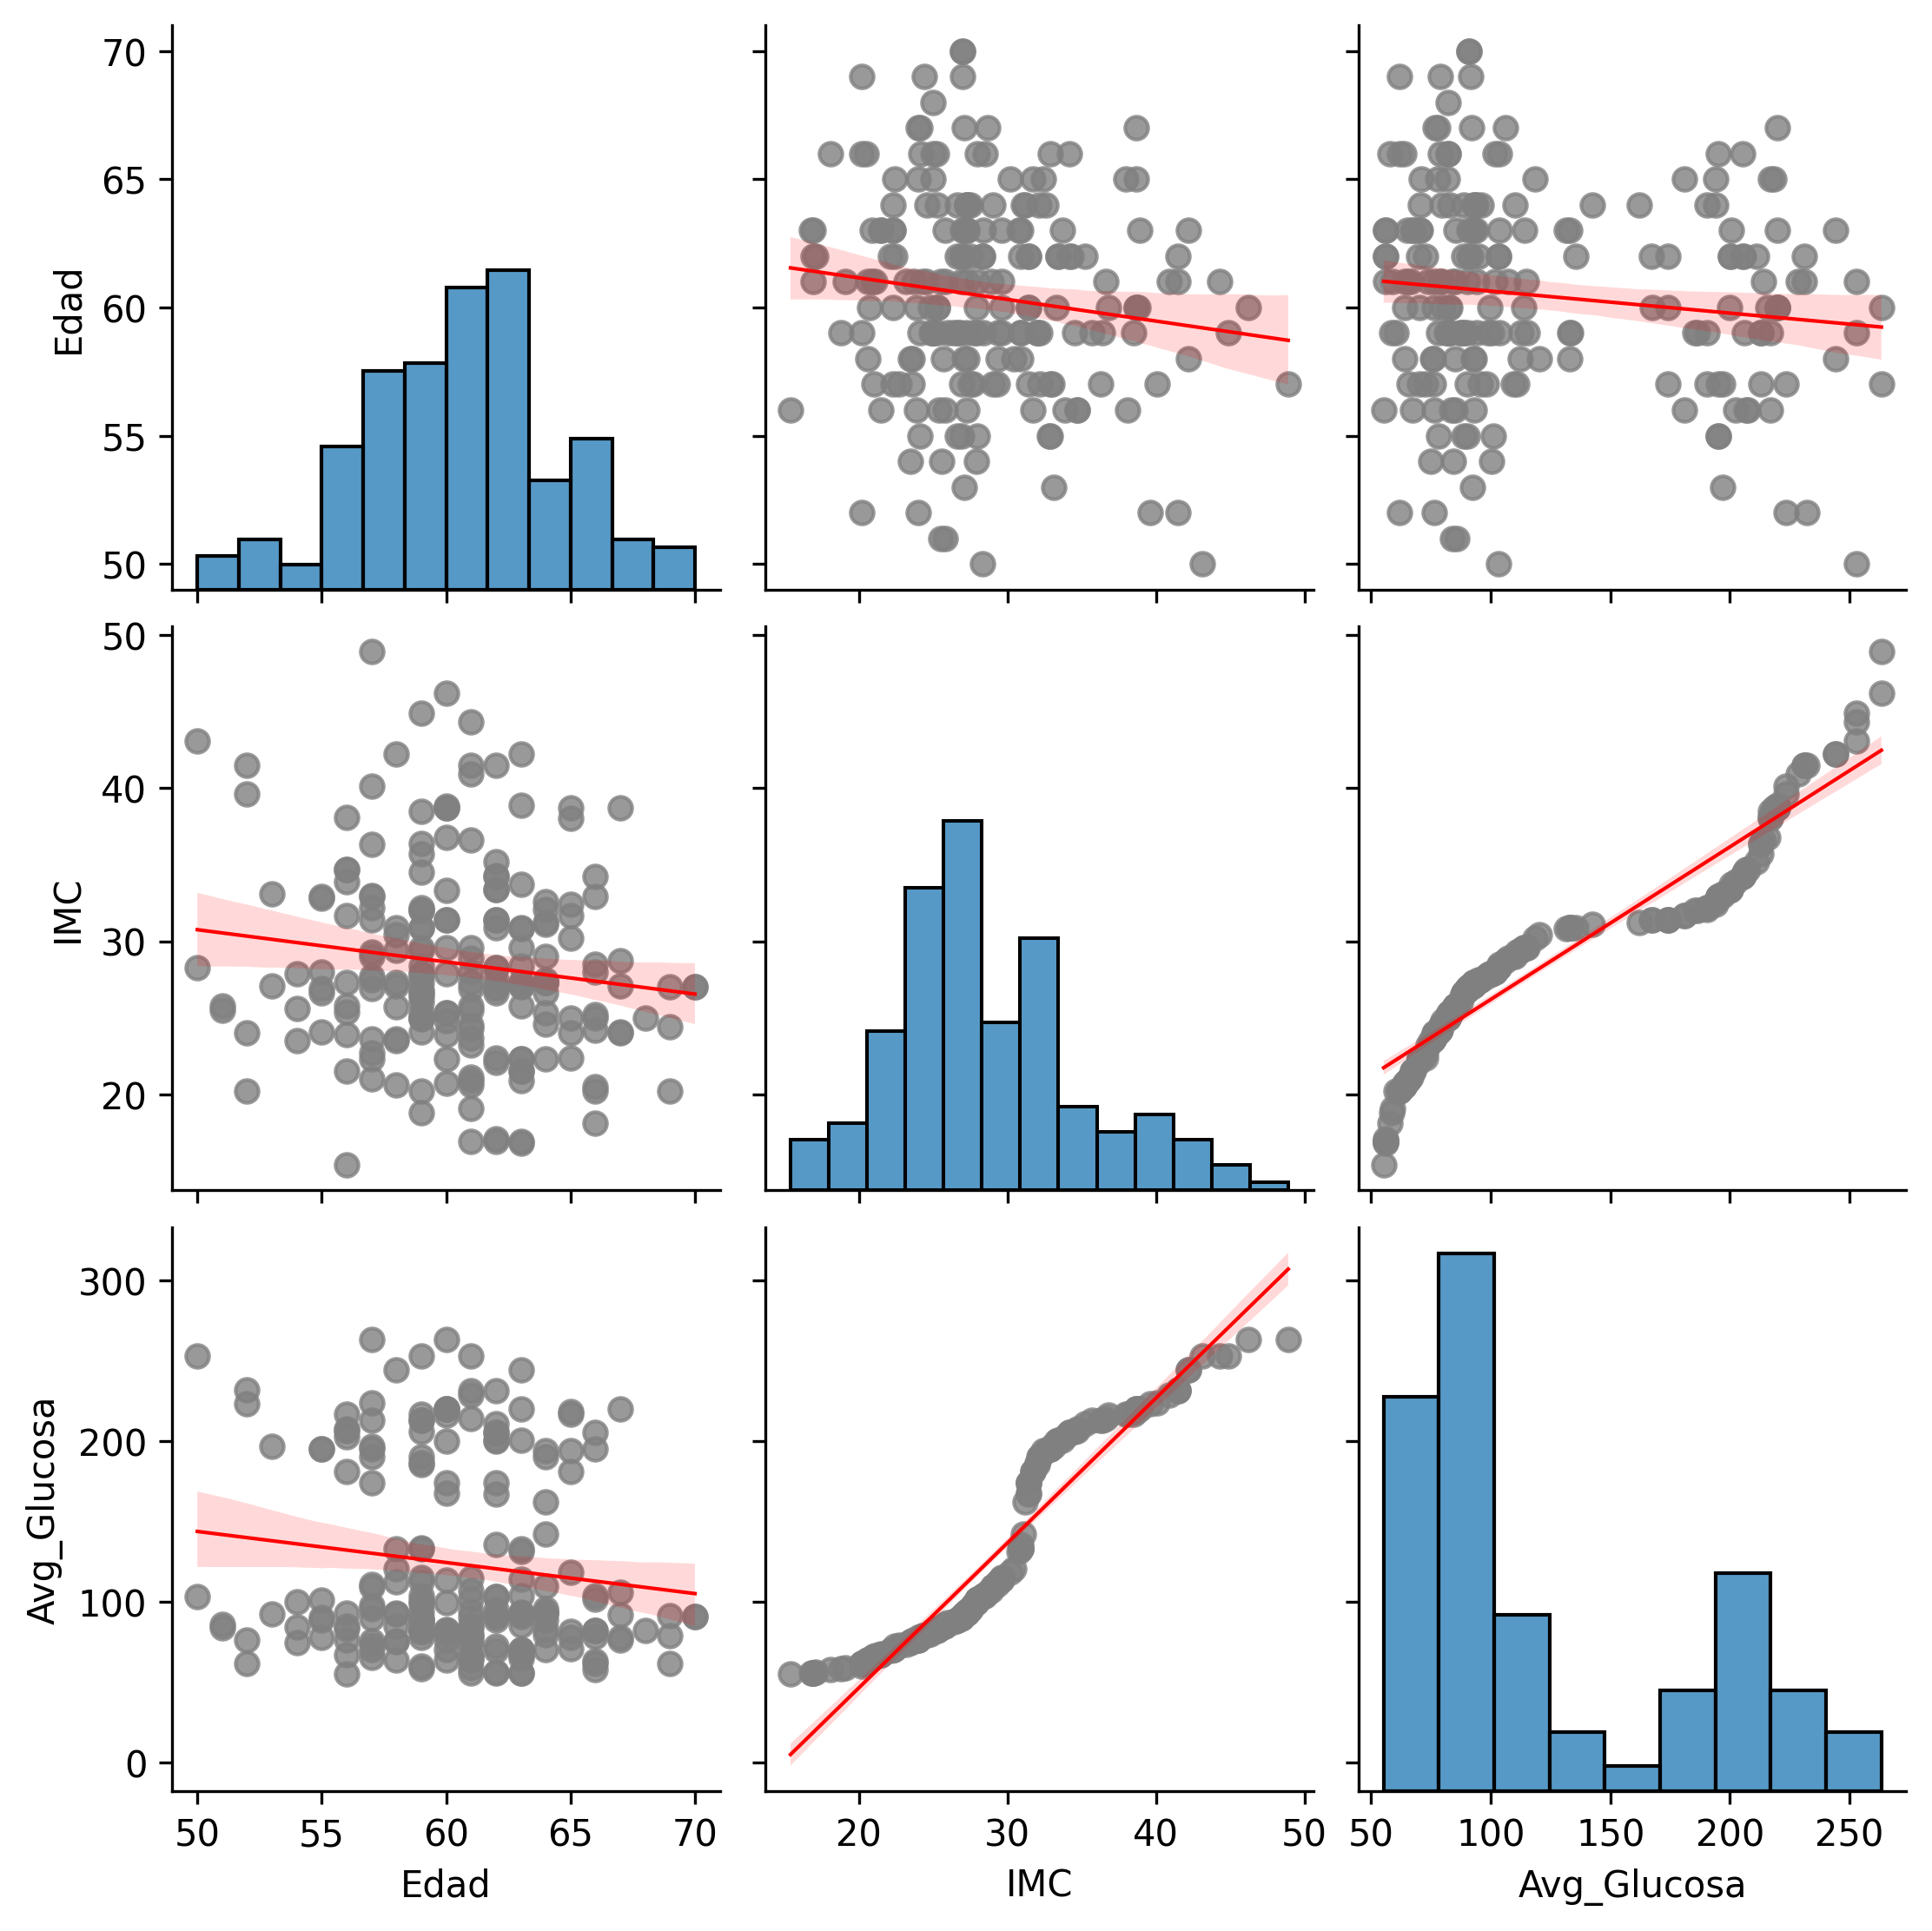
\includegraphics[width=0.9\textwidth]{img/matriz_regresion_lineal.png}
\end{figure}

entender cómo las variables del dataset se relacionan entre sí y para identificar posibles modelos predictivos basados en estas relaciones.



\newpage

\section{Modelos de Regresion logística:}

\section{Modelo de la variable Accidentes}

Para este modelo se tomaron como variables independientes: Sex, Fumar e Hipertension, y como
variable dependiente Accidente.
\\
Accuracy: 0.95
La precisión del modelo es del 95\%, lo que indica que el modelo 
predice correctamente el 95\% de los casos en el conjunto de prueba.
\\
Confusion Matrix:
\[
\begin{bmatrix}
19 & 2 \\
0 & 19
\end{bmatrix}\]

La matriz de confusión muestra:
\\
19 verdaderos negativos (TN): casos donde no hubo accidente y el modelo predijo correctamente.
\\
19 verdaderos positivos (TP): casos donde hubo accidente y el modelo predijo correctamente.
\\
2 falsos positivos (FP): casos donde no hubo accidente pero el modelo predijo que sí.
\\
0 falsos negativos (FN): casos donde hubo accidente pero el modelo predijo que no.

\begin{table}[H]
    \centering
    \begin{tabular}{|c|c|c|c|c|}
        \hline
        Clase & Precisión & Exhaustividad & F1-score & Soporte \\ \hline
        0 & 1.00 & 0.90 & 0.95 & 21 \\ \hline
        1 & 0.90 & 1.00 & 0.95 & 19 \\ \hline
        \textbf{Exactitud} & \multicolumn{4}{c|}{0.95} \\ \hline
        \textbf{Promedio macro} & 0.95 & 0.95 & 0.95 & 40 \\ \hline
        \textbf{Promedio ponderado} & 0.95 & 0.95 & 0.95 & 40 \\ \hline
    \end{tabular}
    \caption{Informe de clasificación}
    \label{tab:classification_report}
\end{table}


Precisión (precision): La precisión para la clase 0 es 1.00 y para la clase 1 es 0.90. Esto significa que el modelo es muy preciso en predecir la clase 0, pero tiene un 10% de error en predecir la clase 1.
\\
Exhaustividad (recall): La exhaustividad para la clase 0 es 0.90 y para la clase 1 es 1.00. Esto significa que el modelo identifica correctamente todos los casos de la clase 1, pero pierde un 10% de los casos de la clase 0.
F1-score: El F1-score es 0.95 para ambas clases, lo que indica un buen equilibrio entre precisión y exhaustividad.

\begin{table}[H]
    \centering
    \begin{tabular}{|c|c|}
        \hline
        Variable & Coeficiente \\ \hline
        Sex & 0.045076 \\ \hline
        Fumar & 4.293324 \\ \hline
        Hipertension & 1.841522 \\ \hline
    \end{tabular}
    \caption{Coeficientes del modelo de regresión logística}
    \label{tab:coeficientes_modelo}
\end{table}

Los coeficientes indican la relación entre cada variable independiente y la probabilidad de que ocurra un Accidente:
\\
Sex: Un coeficiente de 0.045076 sugiere que el sexo tiene un impacto positivo muy pequeño en la probabilidad de accidente.
\\
Fumar: Un coeficiente de 4.293324 indica que fumar aumenta significativamente la probabilidad de accidente.
\\
Hipertension: Un coeficiente de 1.841522 sugiere que la hipertensión también aumenta la probabilidad de accidente, aunque en menor medida que fumar.
\\
Conclusión
El modelo de regresión logística tiene una alta precisión y es capaz de predecir correctamente 
la mayoría de los casos. Las variables Fumar y Hipertension tienen un impacto significativo en 
la probabilidad de accidente, mientras que el Sex tiene un impacto menor.

\section{Modelo de la variable hipertensión}

Para este modelo se tomaron como variables independientes: Sex, Fumar y Edad, y como
variable dependiente Hipertension.


Accuracy: 0.825
La precisión del modelo es del 82.5%, lo que indica que el modelo predice correctamente 
el 82.5% de los casos en el conjunto de prueba. Esto es un buen indicador, aunque hay margen para mejorar.
Confusion Matrix:
[[22  5]
 [ 2 11]]

La matriz de confusión muestra:

22 verdaderos negativos (TN): casos donde no hubo hipertensión y el modelo predijo correctamente.
11 verdaderos positivos (TP): casos donde hubo hipertensión y el modelo predijo correctamente.
5 falsos positivos (FP): casos donde no hubo hipertensión pero el modelo predijo que sí.
2 falsos negativos (FN): casos donde hubo hipertensión pero el modelo predijo que no.

Classification Report:
              precision    recall  f1-score   support

           0       0.92      0.81      0.86        27
           1       0.69      0.85      0.76        13

    accuracy                           0.82        40
   macro avg       0.80      0.83      0.81        40
weighted avg       0.84      0.82      0.83        40

Precisión (precision): La precisión para la clase 0 es 0.92 y para la clase 1 es 0.69. Esto significa que el modelo es más preciso en predecir la clase 0 que la clase 1.
Exhaustividad (recall): La exhaustividad para la clase 0 es 0.81 y para la clase 1 es 0.85. Esto significa que el modelo identifica correctamente el 85% de los casos de la clase 1.
F1-score: El F1-score es 0.86 para la clase 0 y 0.76 para la clase 1, lo que indica un buen equilibrio entre precisión y exhaustividad.

Coeficientes del modelo:
  Variable  Coeficiente
0      Sex    -0.567660
1    Fumar     3.493276
2     Edad    -0.066406

Los coeficientes indican la relación entre cada variable independiente y la probabilidad de hipertensión:

Sex: Un coeficiente de -0.567660 sugiere que el sexo tiene un impacto negativo en la probabilidad de hipertensión.
Fumar: Un coeficiente de 3.493276 indica que fumar aumenta significativamente la probabilidad de hipertensión.
Edad: Un coeficiente de -0.066406 sugiere que la edad tiene un impacto negativo muy pequeño en la probabilidad de hipertensión.


\newpage

\section{Gráficos de pastel}
A continuación visualizaremos la proporcion en la que aparecen las variables cualitativas respecto del total

\begin{figure}[H]
    \centering
    \begin{minipage}{0.45\textwidth}
        \centering
        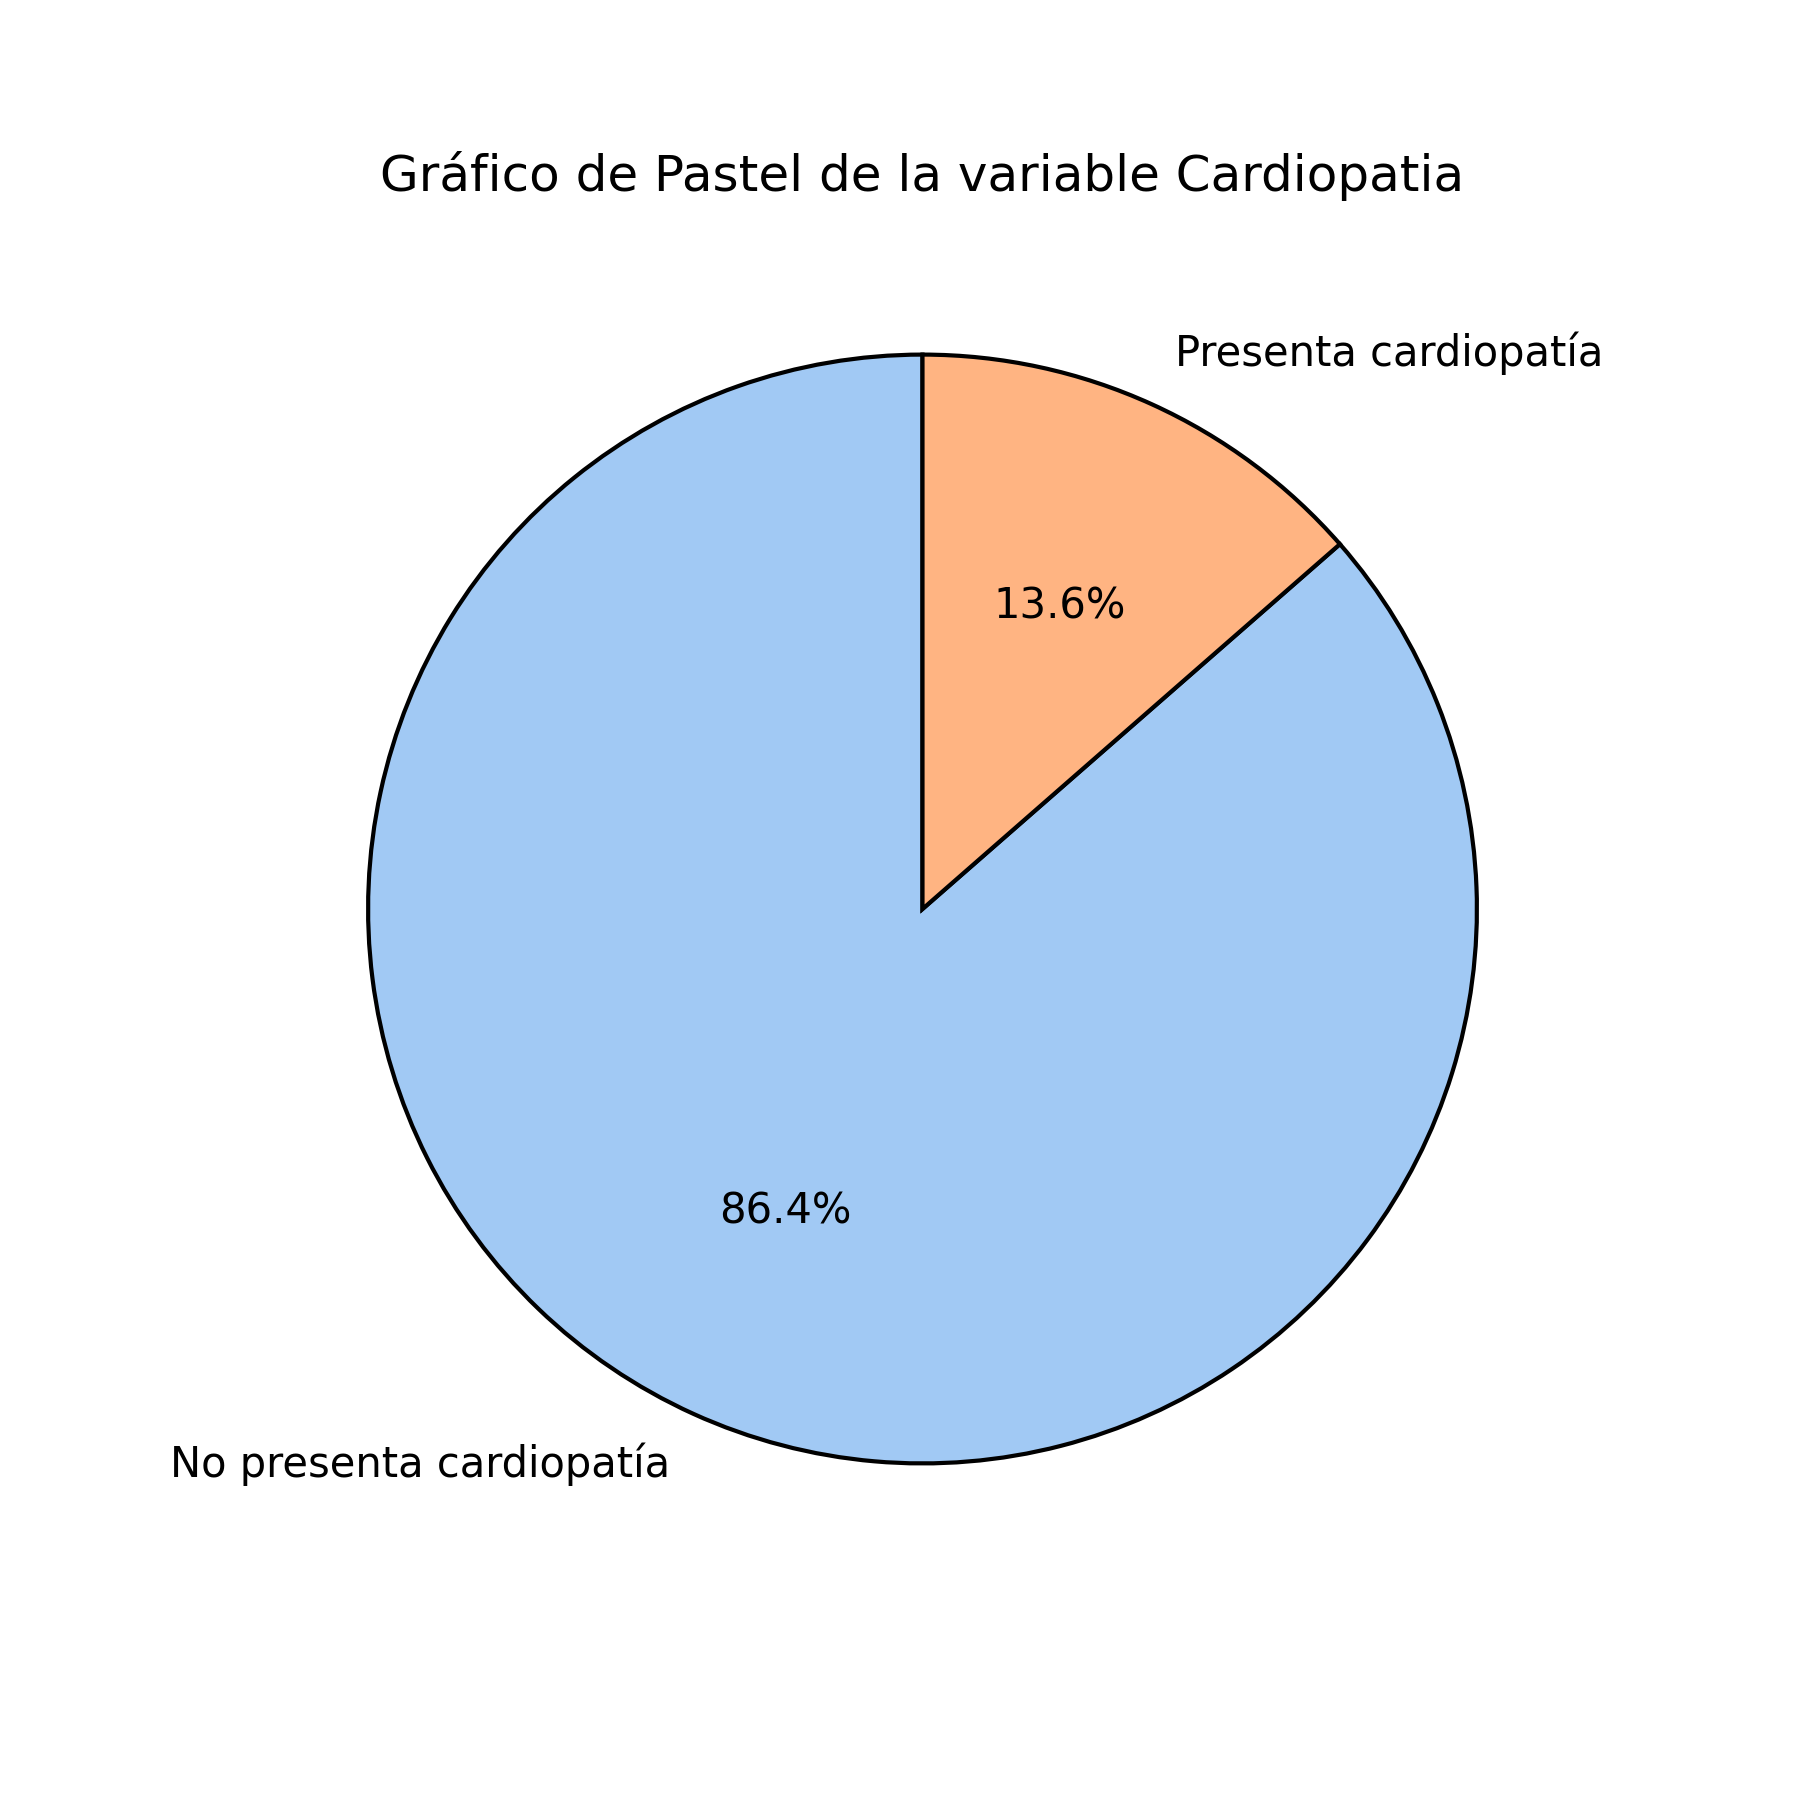
\includegraphics[width=0.9\textwidth]{img/GráficosPastel/grafico_pastel_Cardiopatia.png}
    \end{minipage}
    \begin{minipage}{0.45\textwidth}
        \centering
        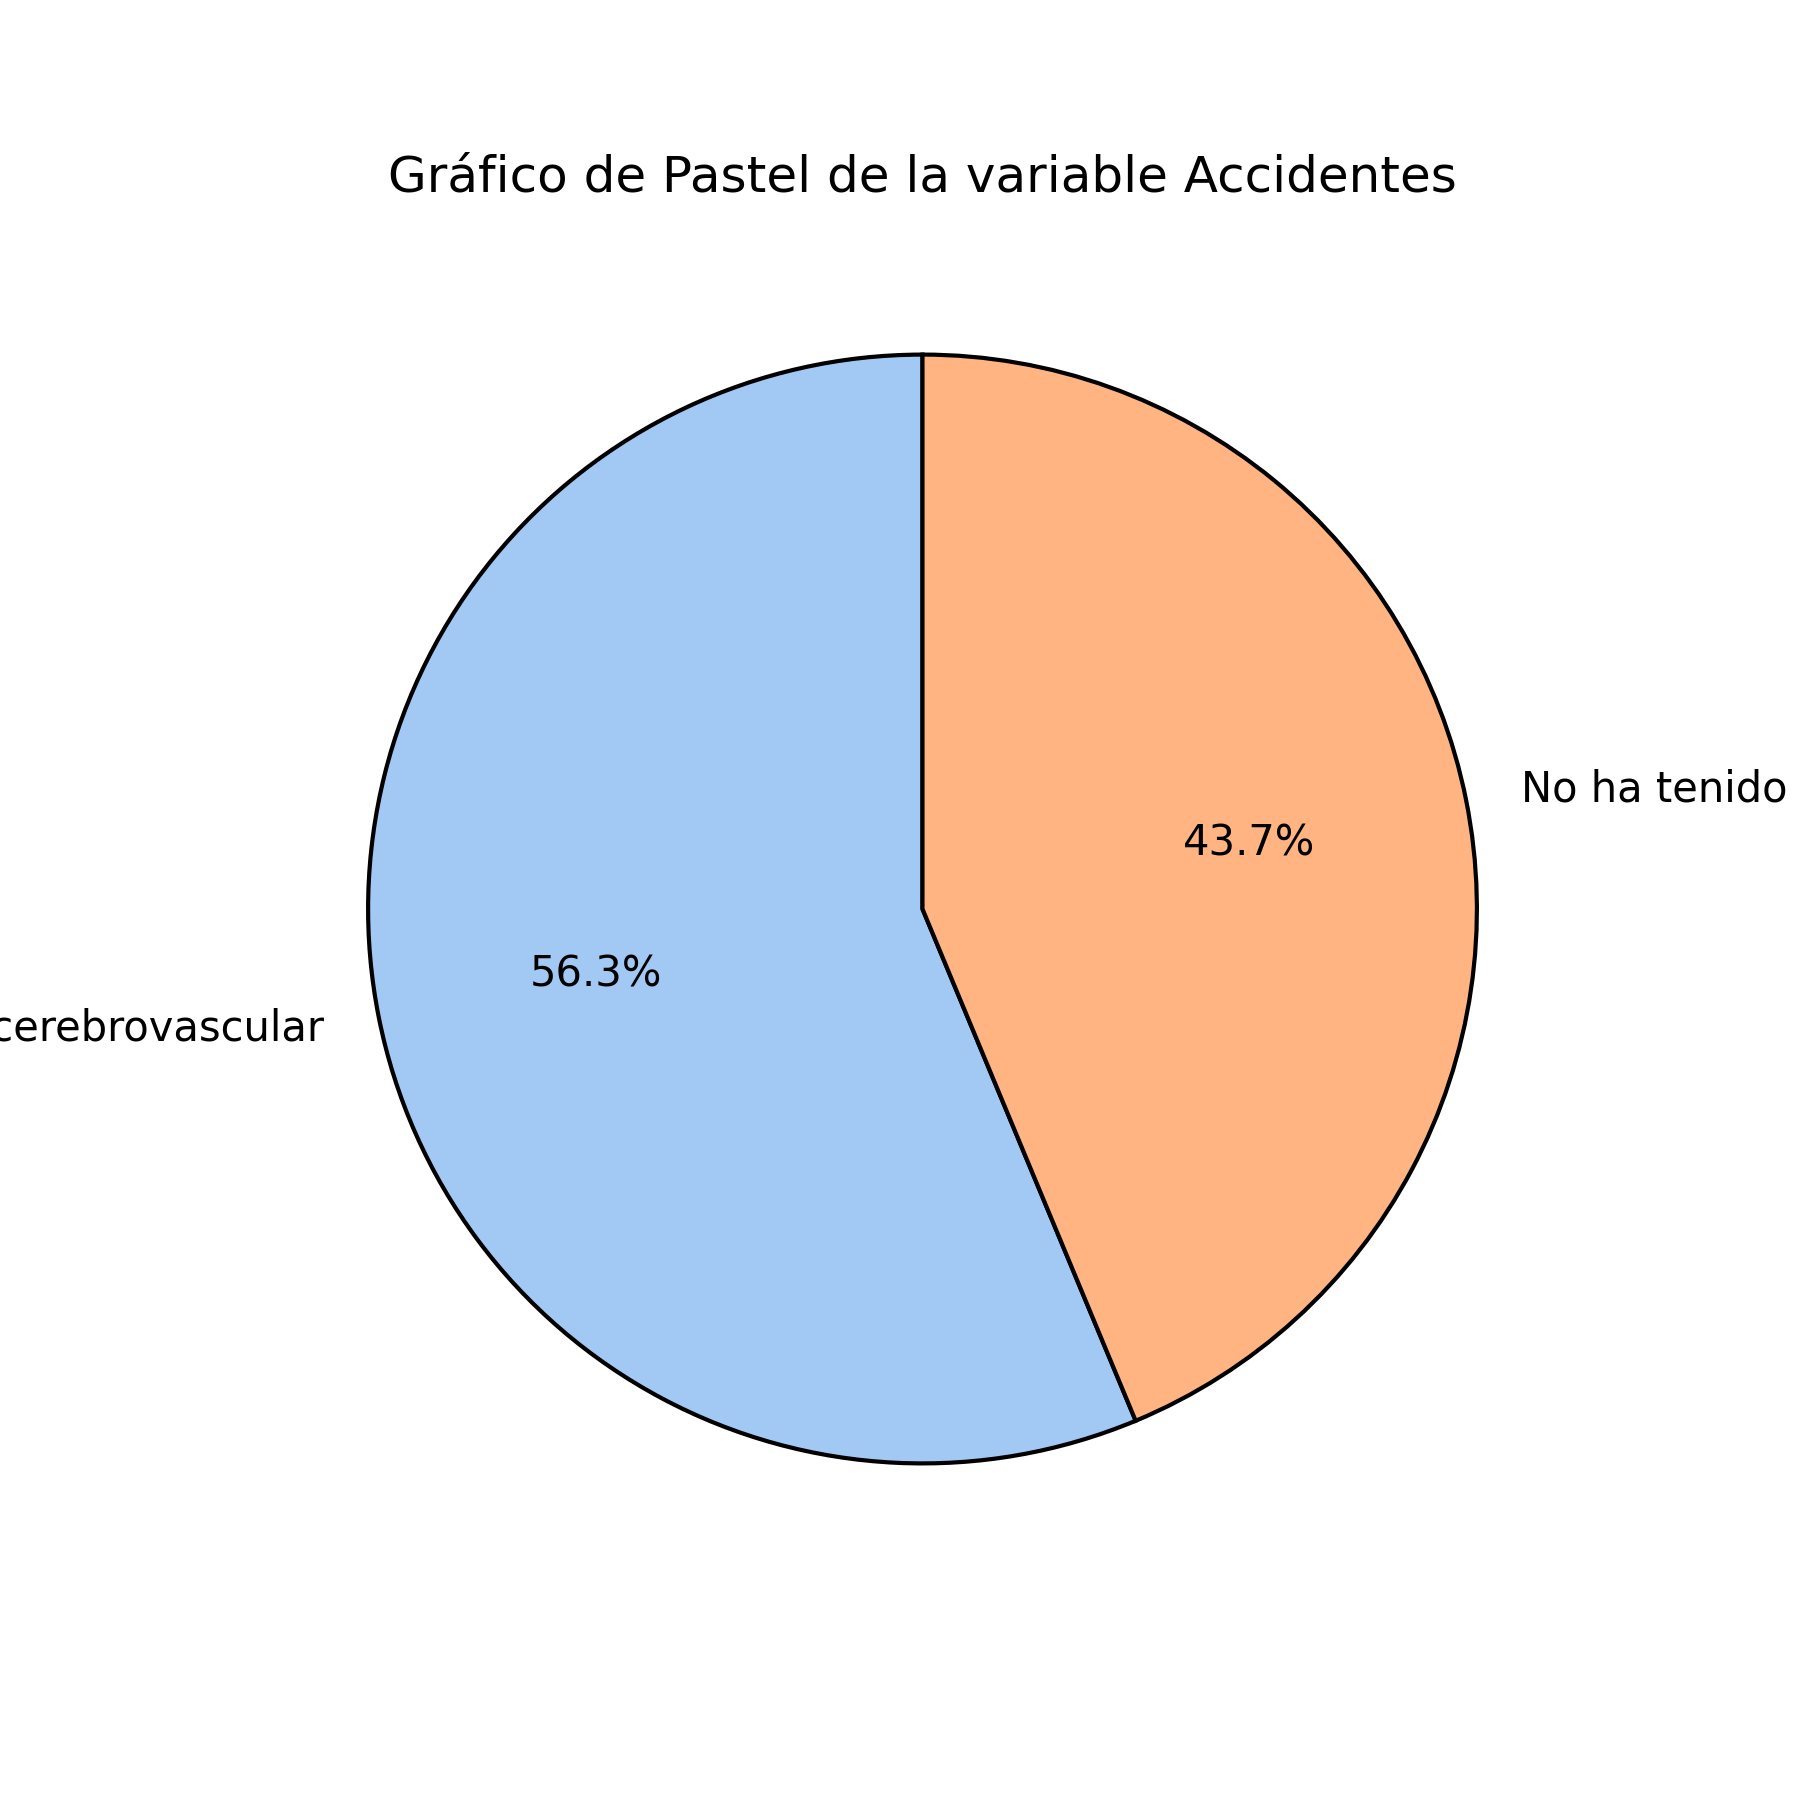
\includegraphics[width=0.9\textwidth]{img/GráficosPastel/grafico_pastel_Accidentes.png}
    \end{minipage}
    \vfill
    \begin{minipage}{0.45\textwidth}
        \centering
        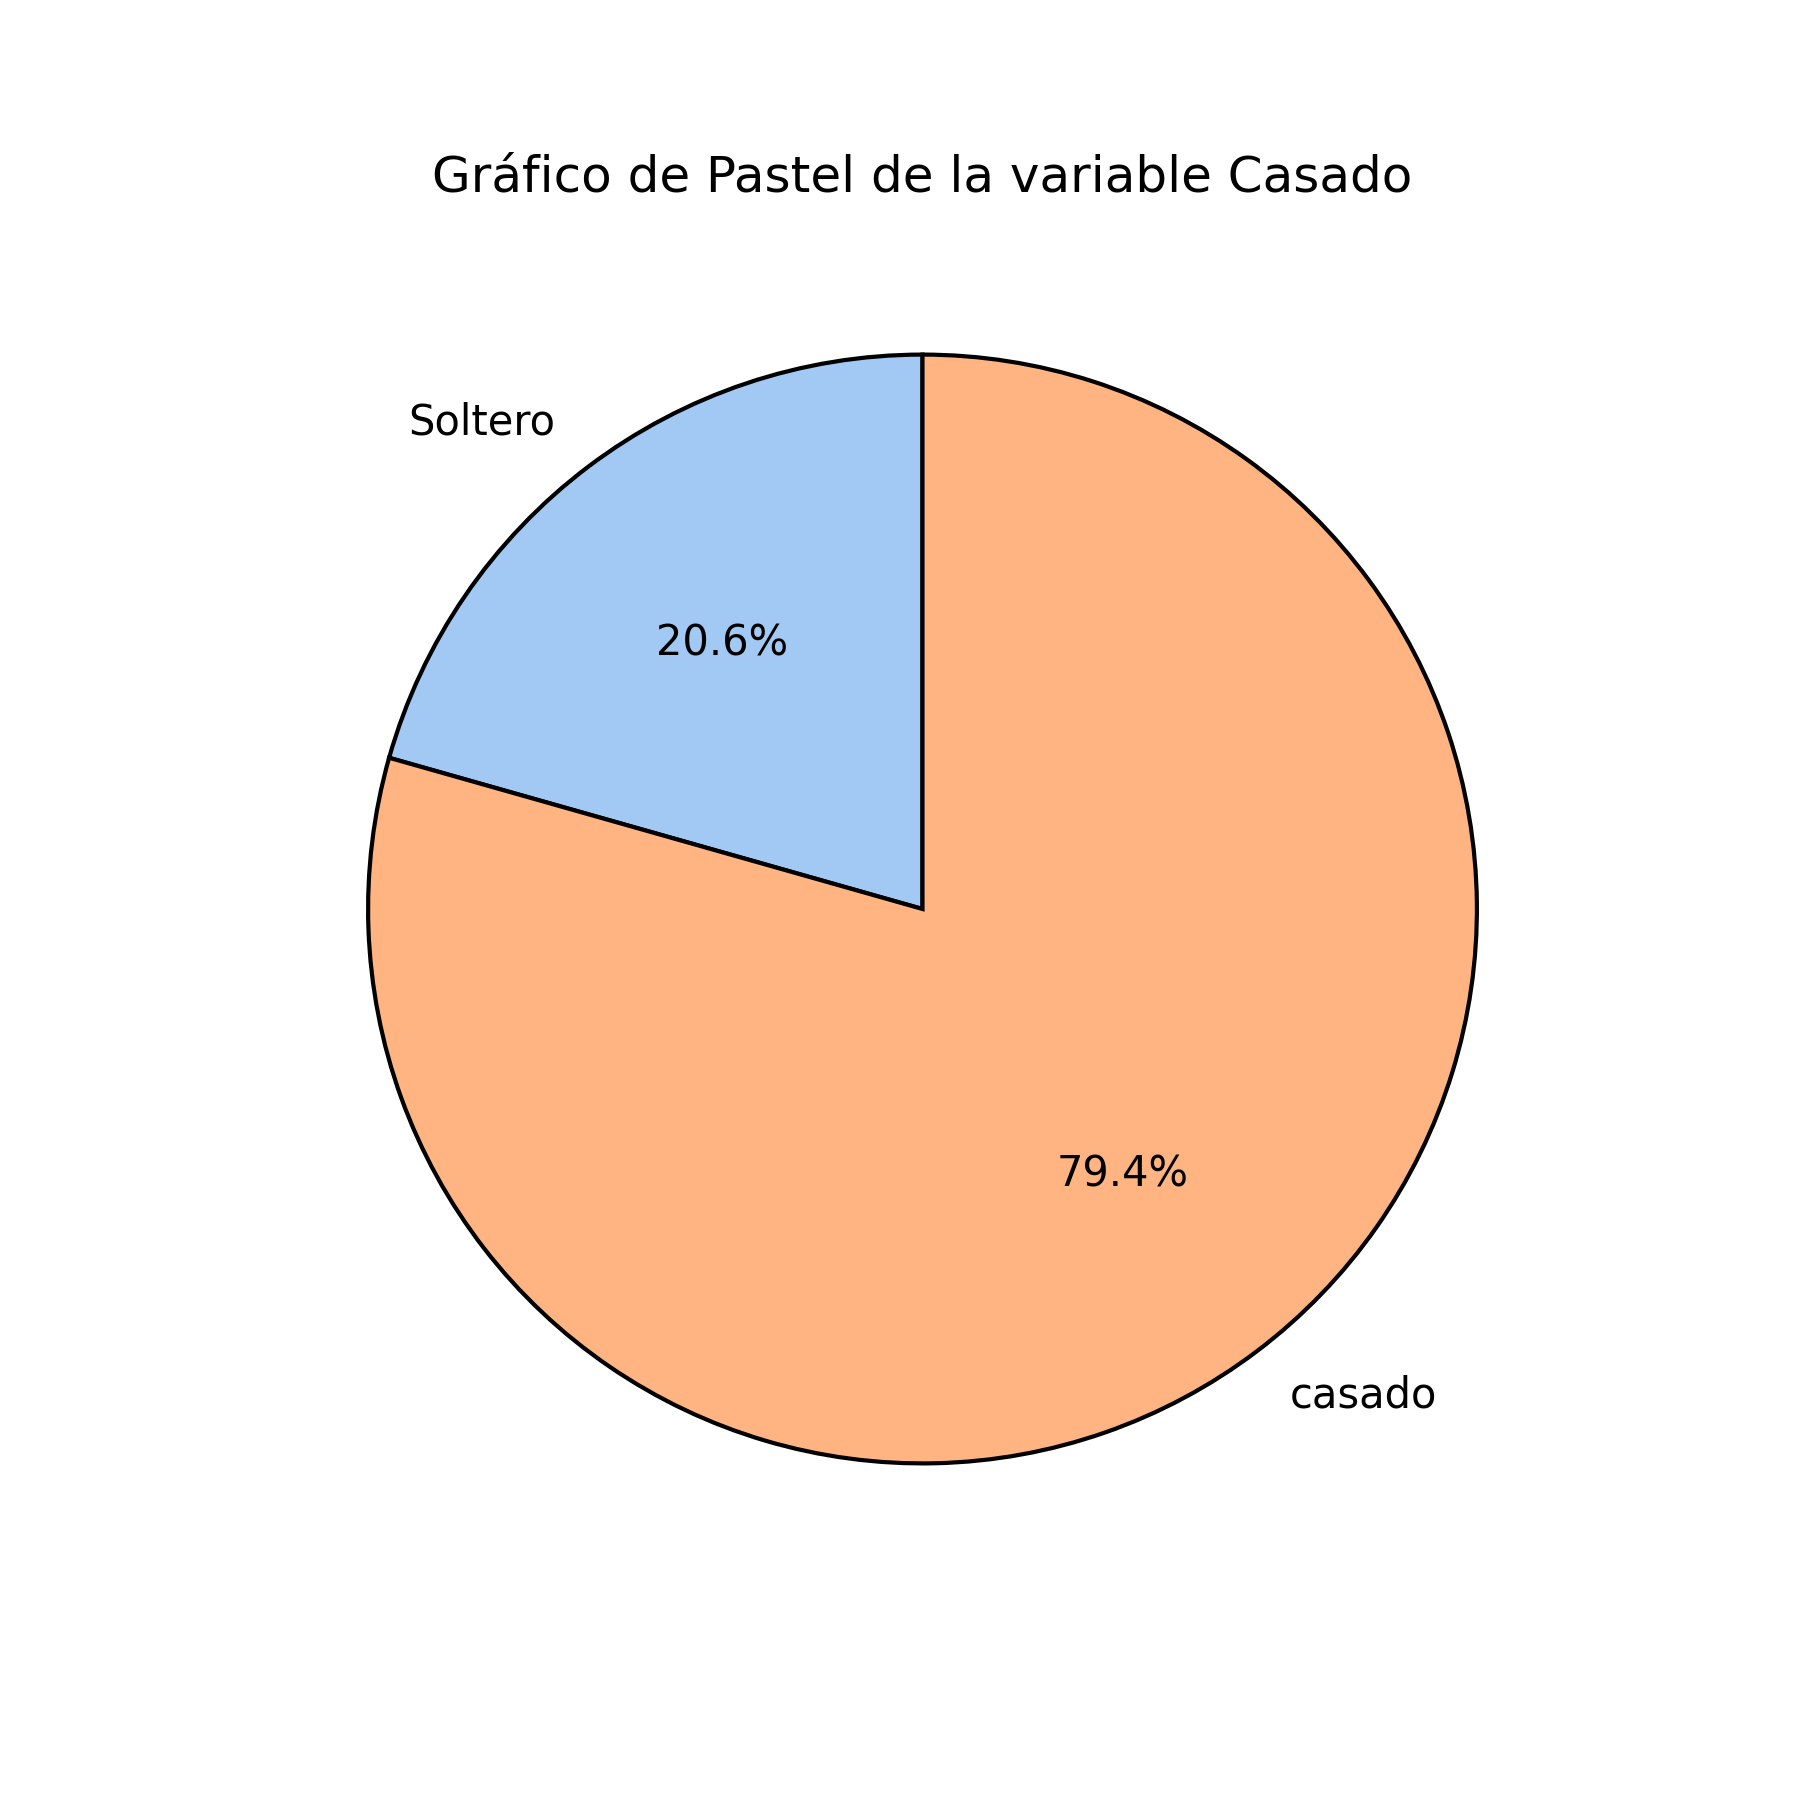
\includegraphics[width=0.9\textwidth]{img/GráficosPastel/grafico_pastel_Casado.png}
    \end{minipage}
    \begin{minipage}{0.45\textwidth}
        \centering
        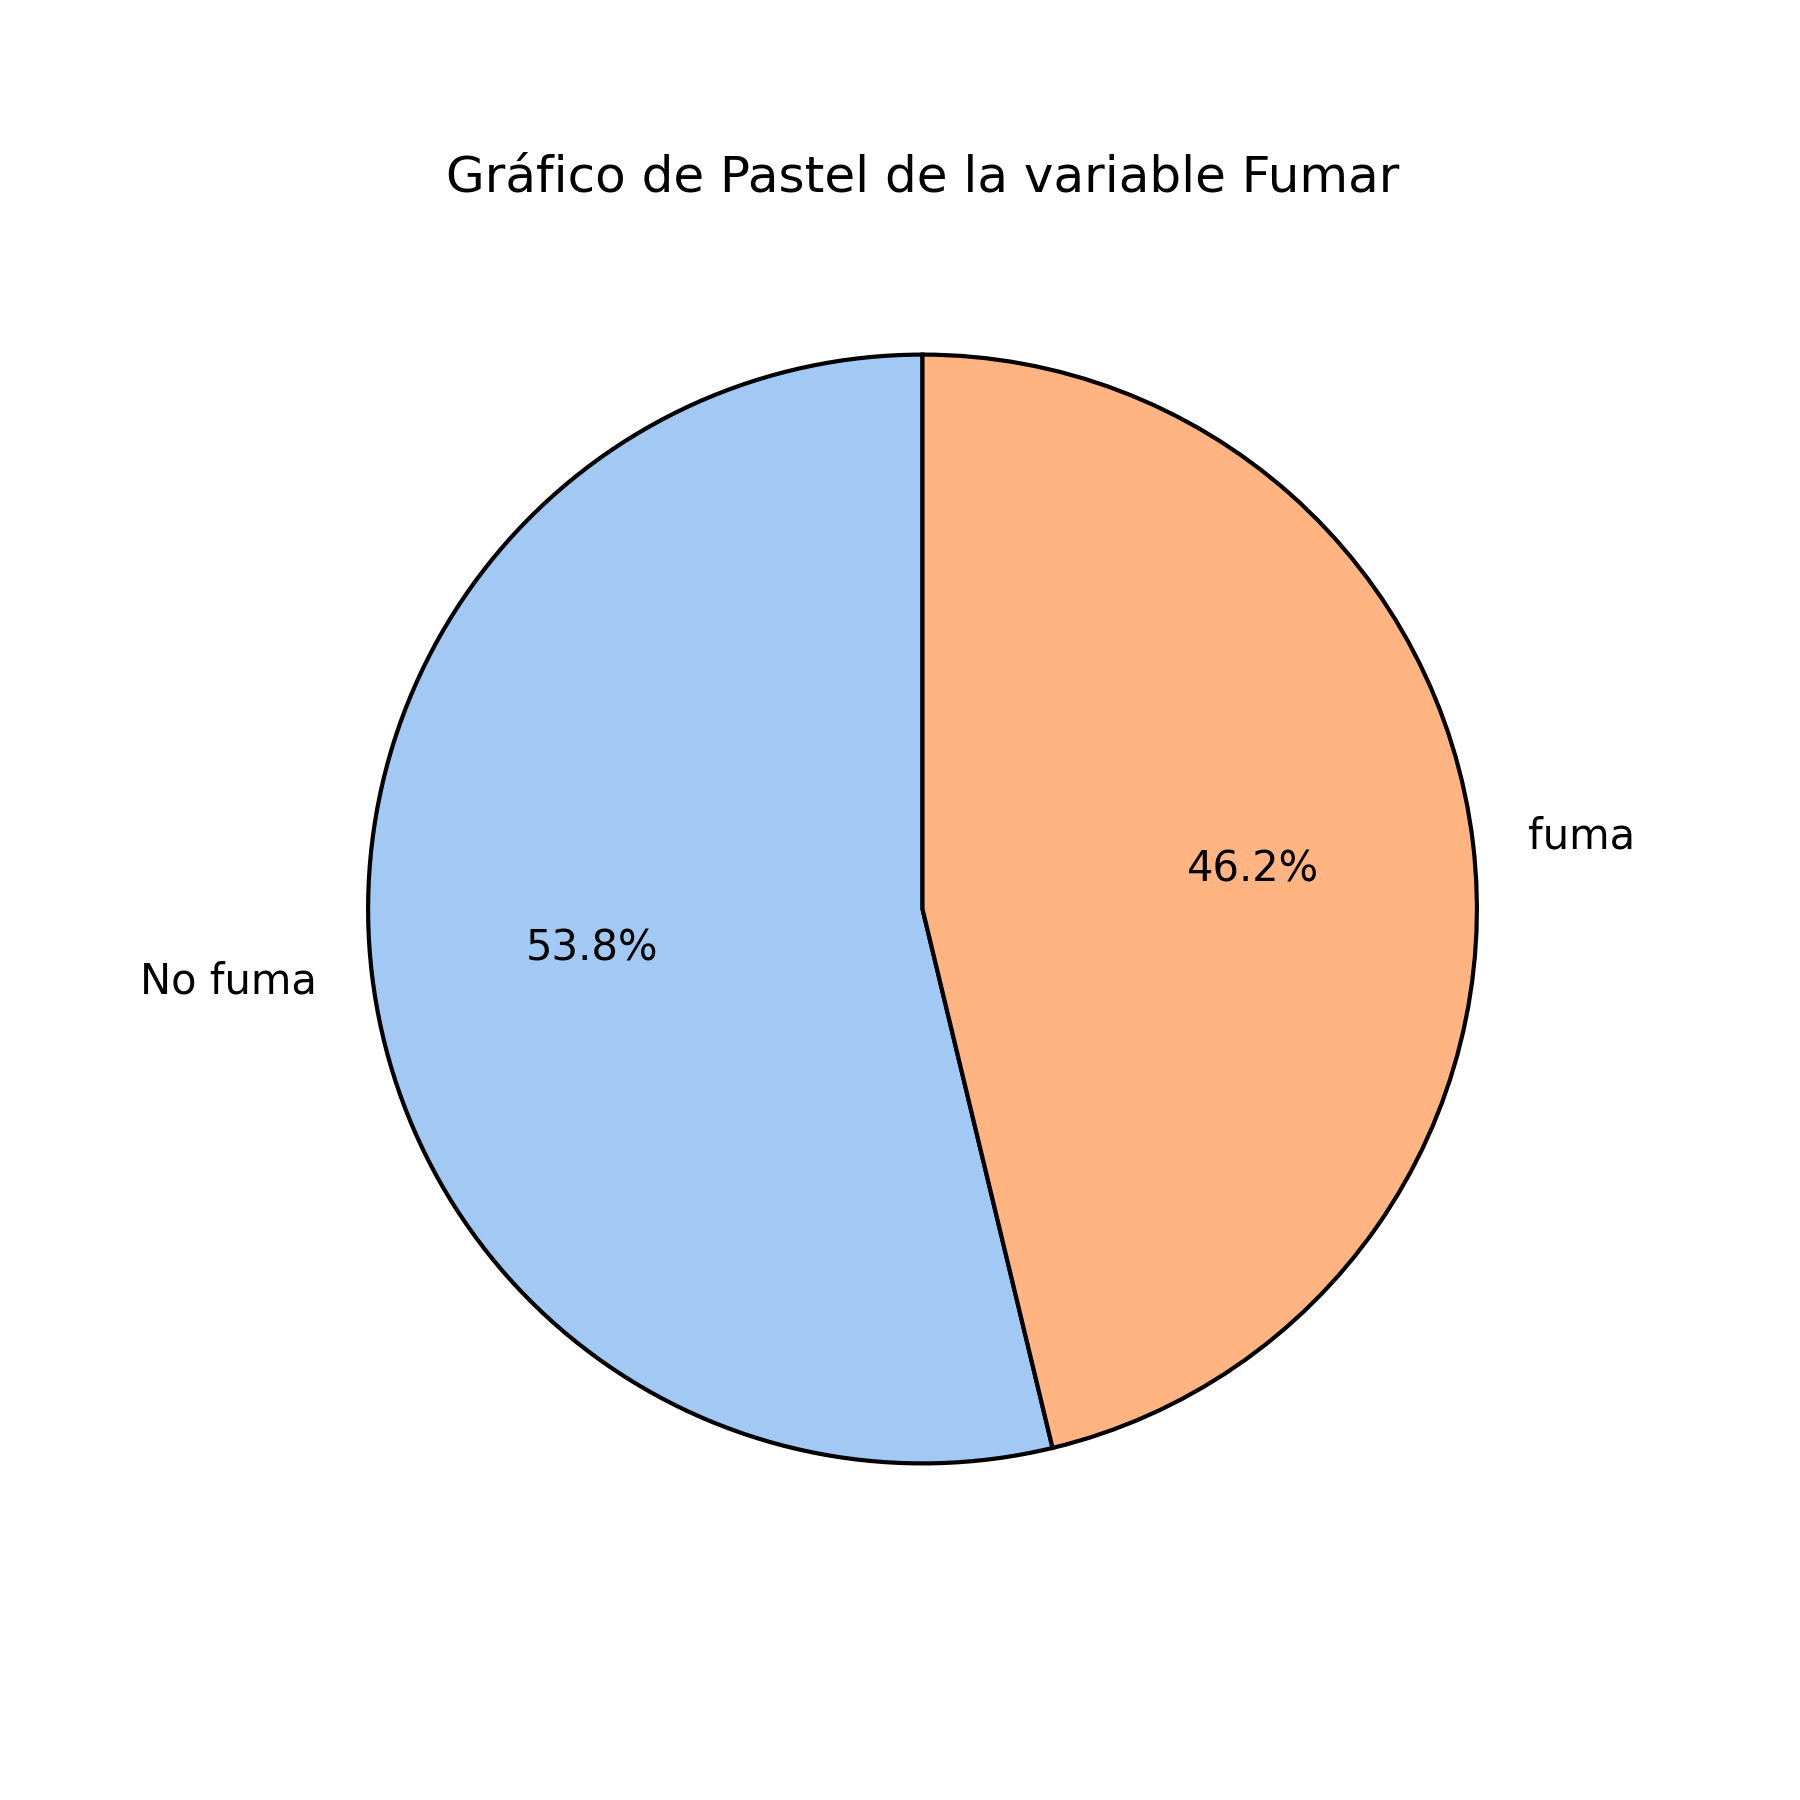
\includegraphics[width=0.9\textwidth]{img/GráficosPastel/grafico_pastel_Fumar.png}
    \end{minipage}
    \vfill
    \begin{minipage}{0.45\textwidth}
        \centering
        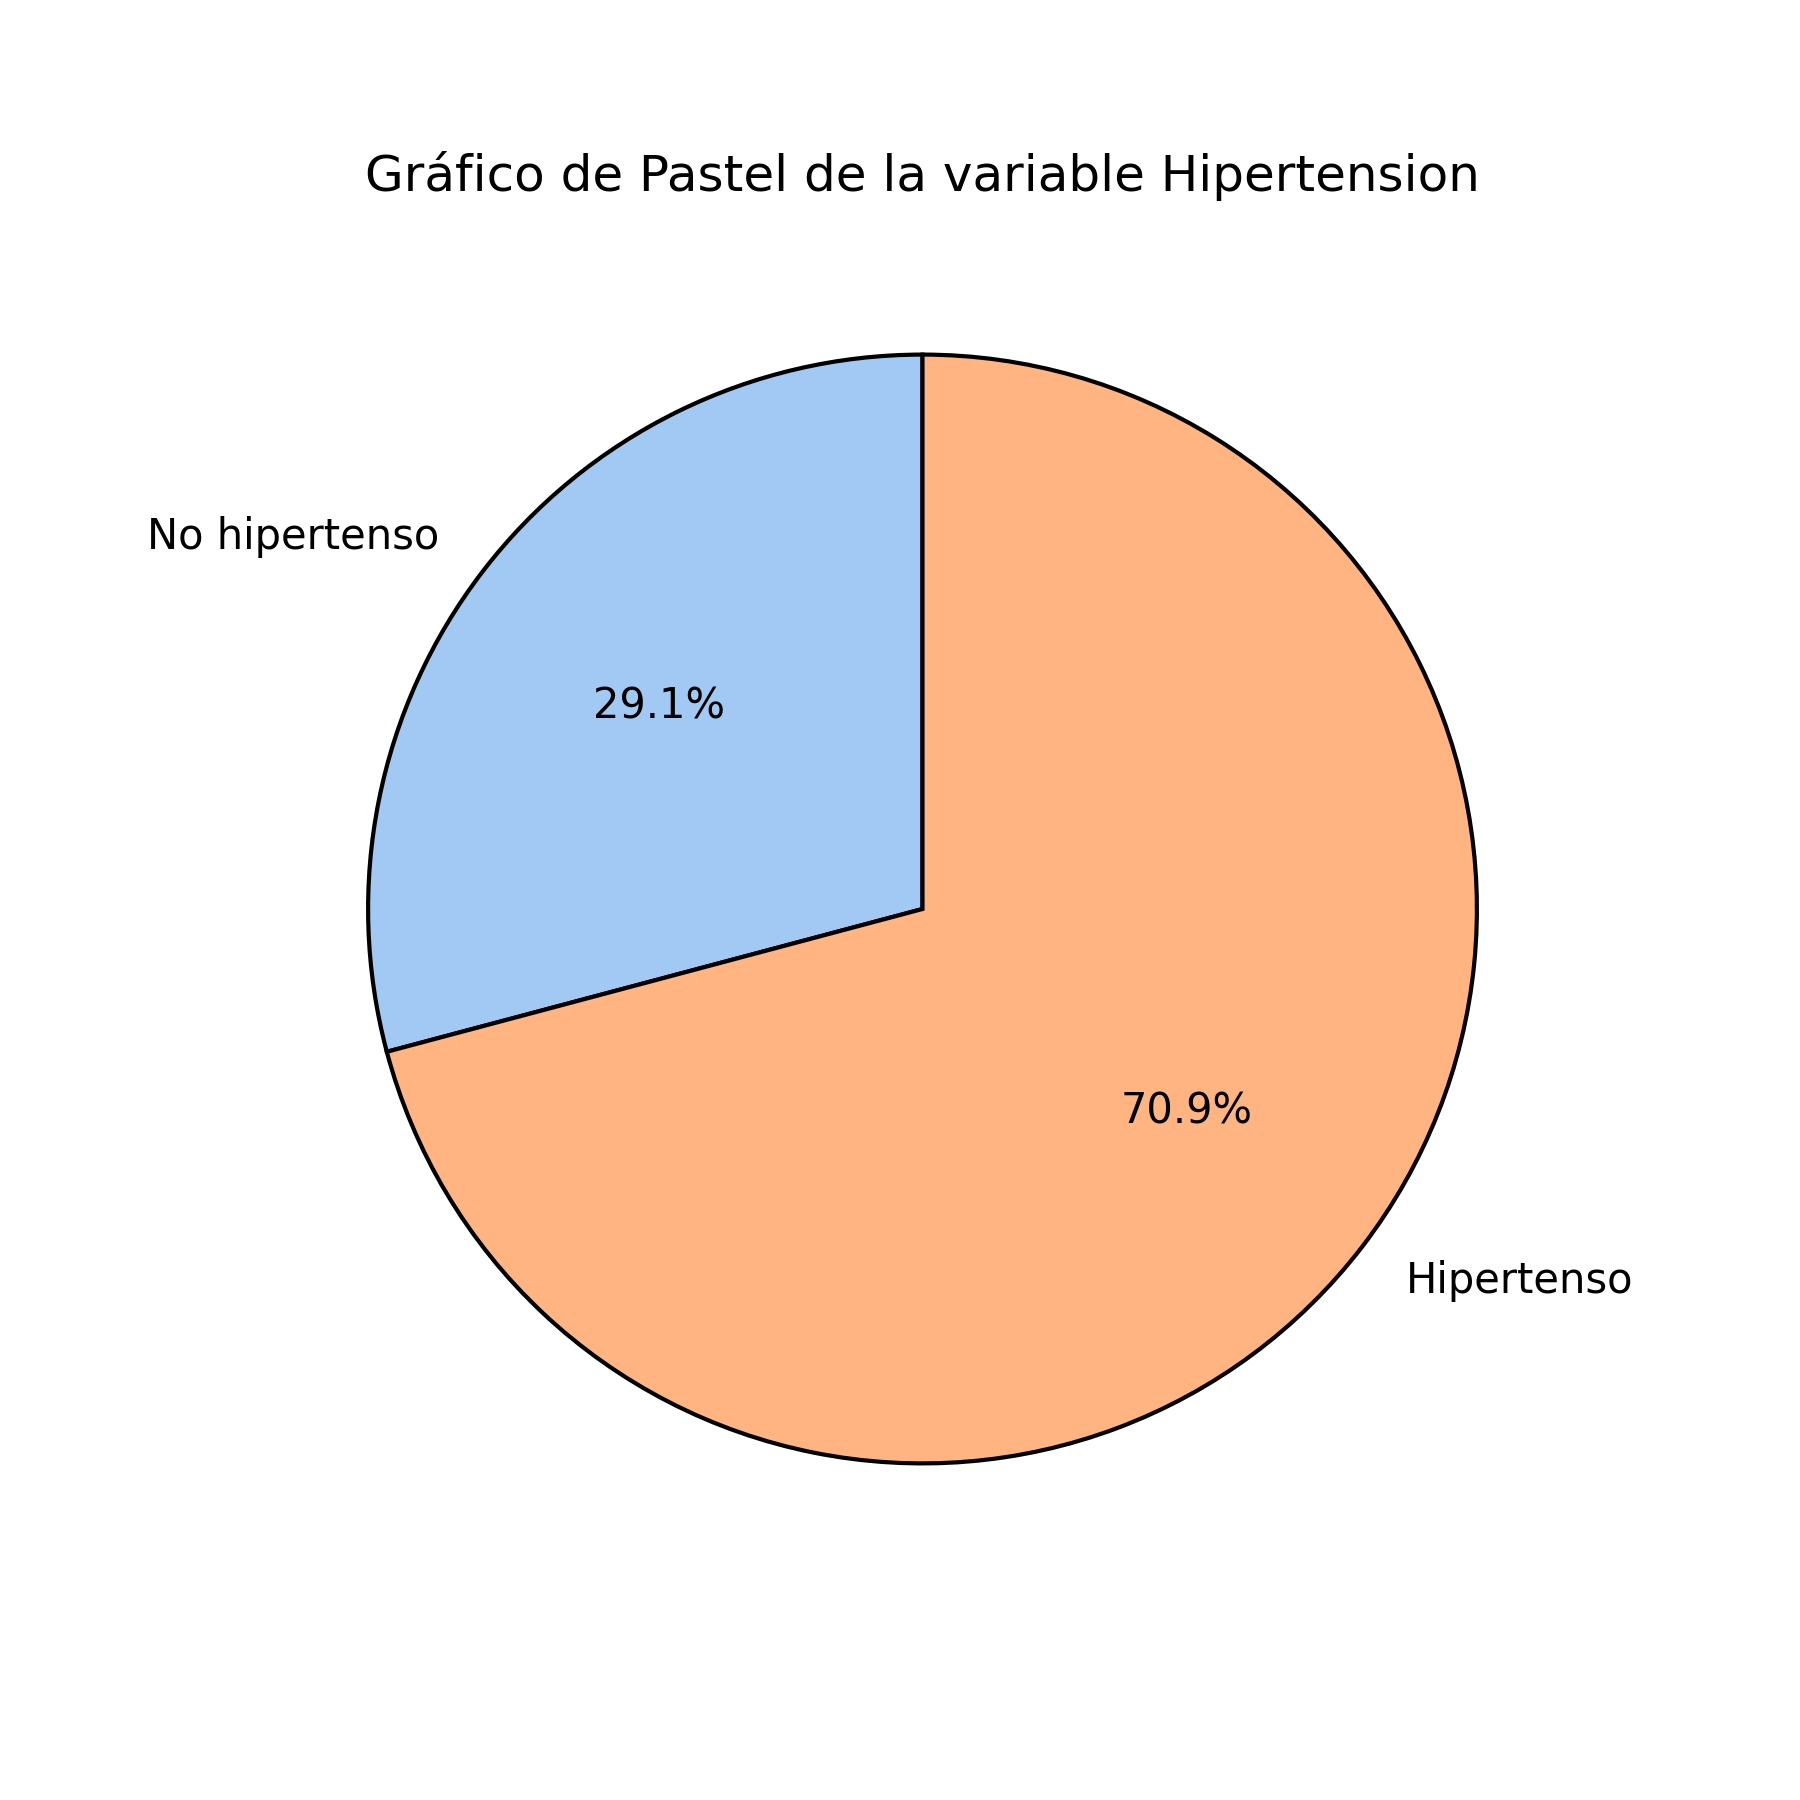
\includegraphics[width=0.9\textwidth]{img/GráficosPastel/grafico_pastel_Hipertension.png}
    \end{minipage}
    \begin{minipage}{0.45\textwidth}
        \centering
        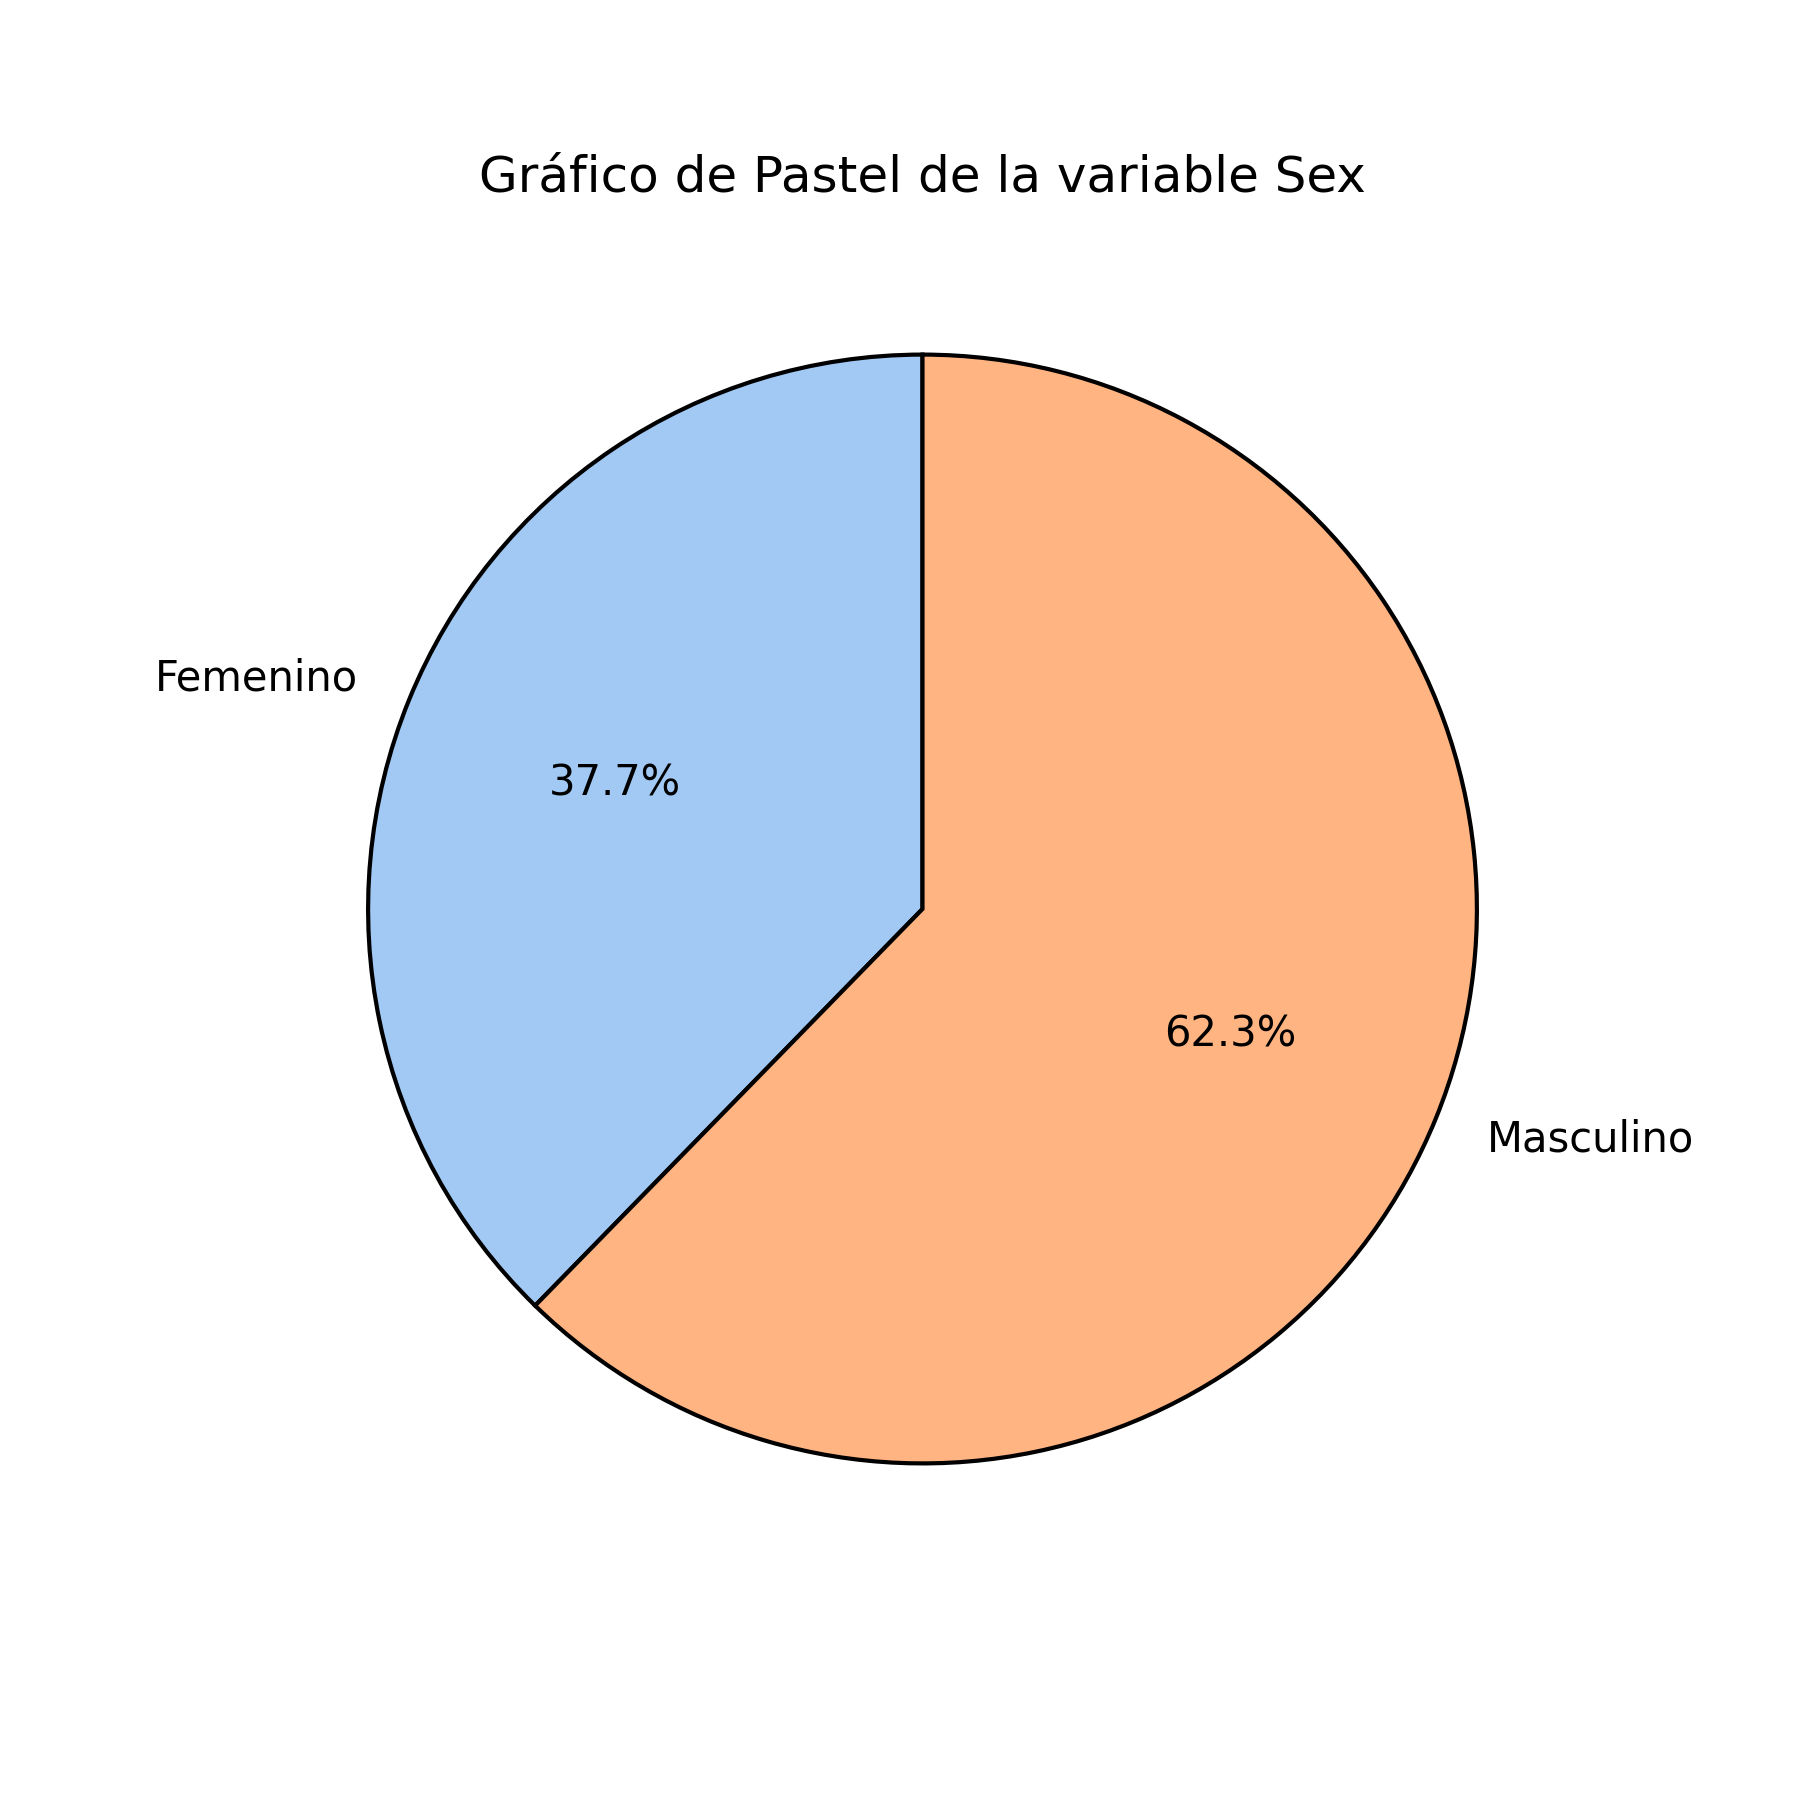
\includegraphics[width=0.9\textwidth]{img/GráficosPastel/grafico_pastel_Sex.png}
    \end{minipage}
    \vfill
    % \begin{minipage}{0.45\textwidth}
    %     \centering
    %     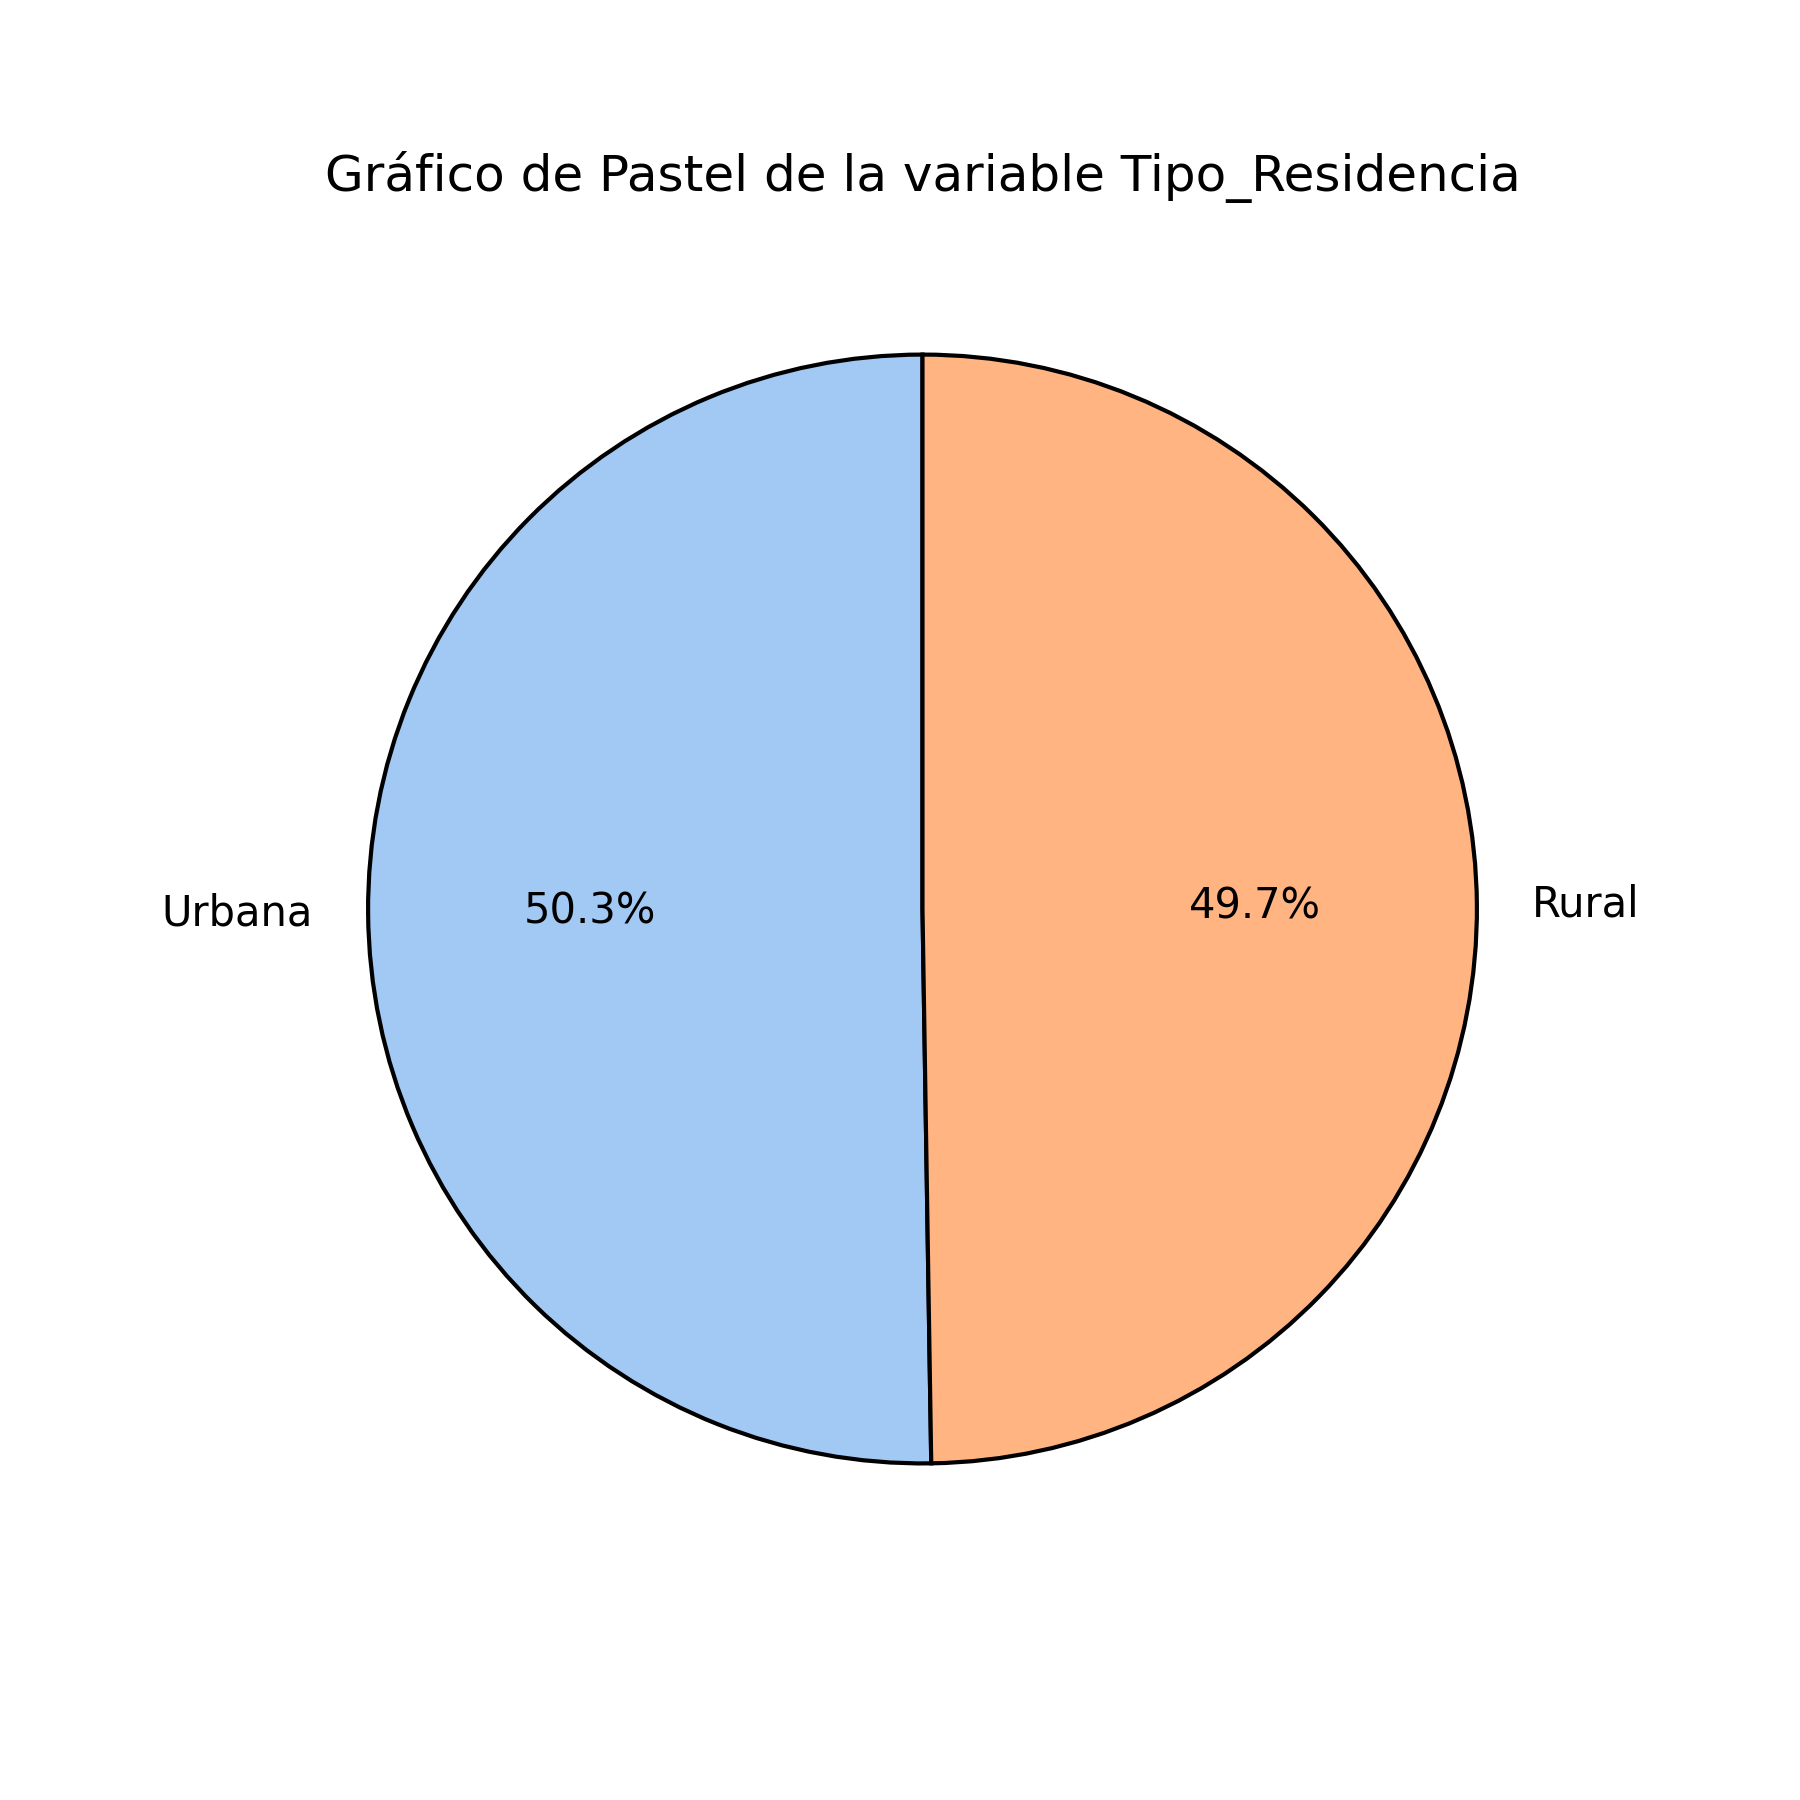
\includegraphics[width=0.3\textwidth]{img/grafico_pastel_Tipo_Residencia.png}
    % \end{minipage}
    % \begin{minipage}{0.45\textwidth}
    %     \centering
    %     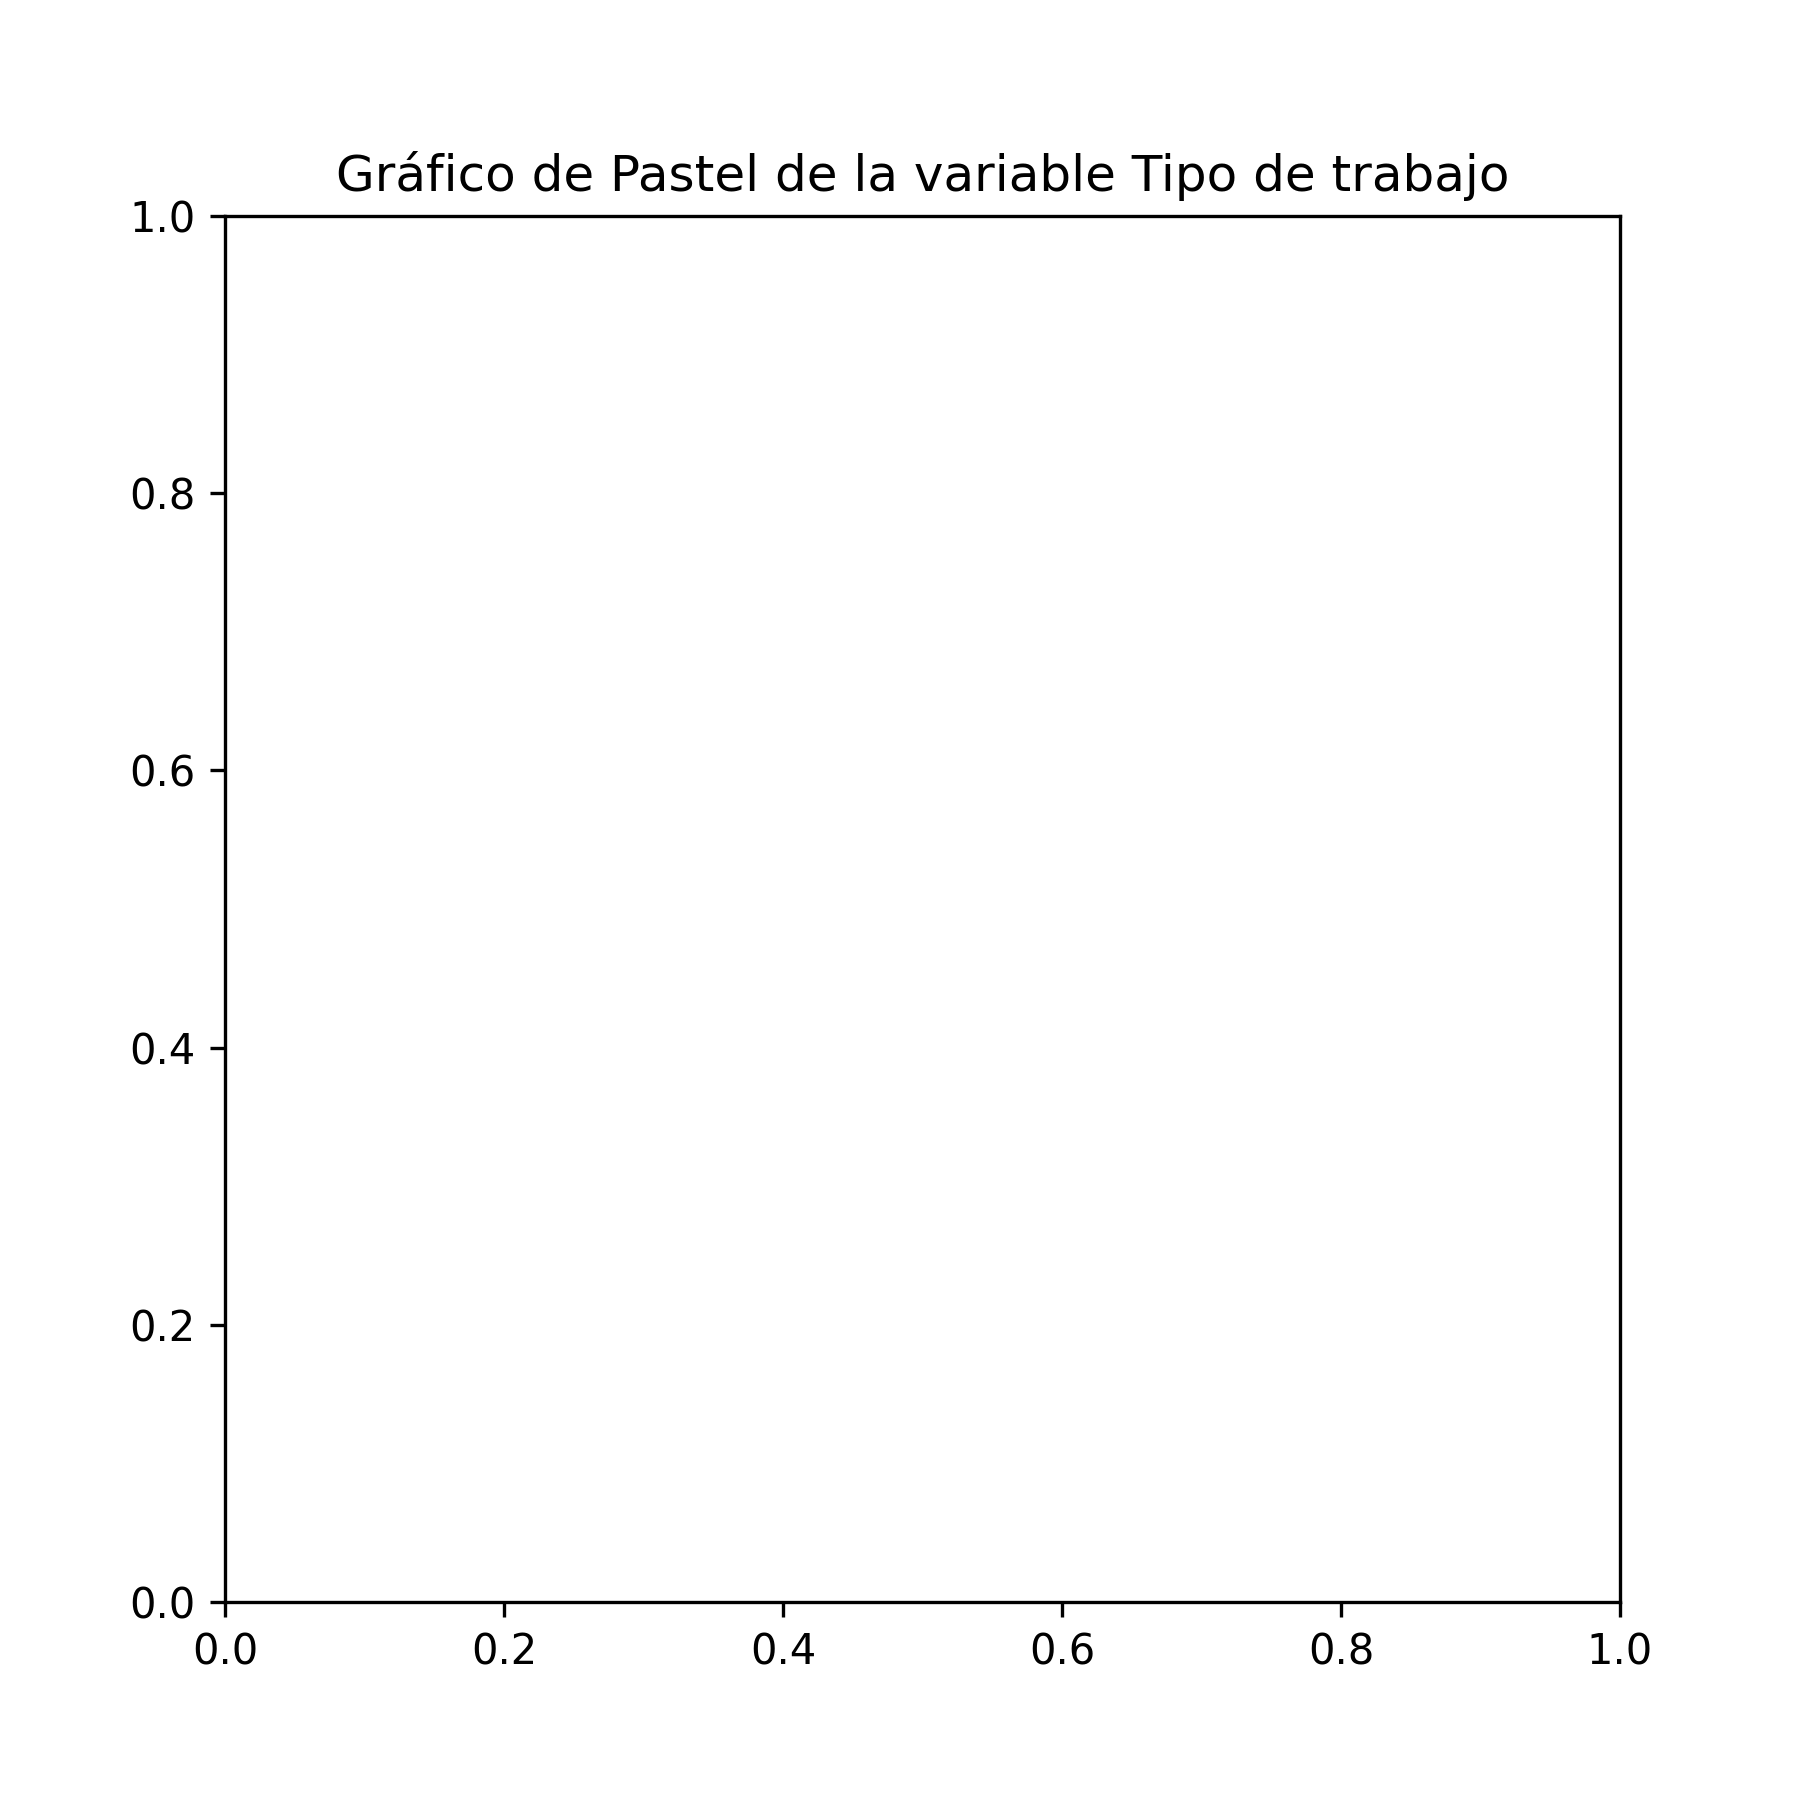
\includegraphics[width=\textwidth]{img/grafico_pastel_Tipo_Trabajo.png.jpg}
    % \end{minipage}
\end{figure}

\end{document}